\documentclass[final,5p,times,authoryear,twocolumn]{elsarticle}

% =========================================================================
% PACKAGES AND FLOAT LAYOUT TUNING
% =========================================================================
\usepackage{amsmath,amssymb,amsfonts}
\usepackage{graphicx}
\usepackage{booktabs}
\usepackage{multirow}
\usepackage{siunitx}
\usepackage[hidelinks]{hyperref}
\usepackage{subcaption}
\usepackage{float}
\usepackage{placeins}

\renewcommand{\topfraction}{0.90}
\renewcommand{\bottomfraction}{0.90}
\renewcommand{\textfraction}{0.08}
\renewcommand{\floatpagefraction}{0.75}
\setcounter{topnumber}{2}
\setcounter{bottomnumber}{2}
\setcounter{totalnumber}{4}

\graphicspath{{figures/}}

\journal{Electric Power Systems Research}

\begin{document}

\begin{frontmatter}

\title{Thermodynamic- and Calendar-Aware Deep Ensembles for National and Divisional Peak Electricity Demand Forecasting in Bangladesh}

\author[nsu]{Mubtasim Fuad}
\ead{mubtasim.fuad@northsouth.edu}
\author[nsu]{Tanvir Anjum Abid}
\ead{tanvir.abid@northsouth.edu}
\author[nsu]{Payel Das}
\ead{payel.das@northsouth.edu}
\author[nsu]{Md. Imam Hossain Rakib}
\ead{imam.rakib@northsouth.edu}
\author[nsu]{Mohammad Rashedur Rahman\corref{cor1}}
\ead{rashedur.rahman@northsouth.edu}

\cortext[cor1]{Corresponding author.}
\address[nsu]{Department of Electrical and Computer Engineering, North South University, Dhaka, Bangladesh}

\begin{abstract}
Accurate short-term load forecasting (STLF) is critical for economic unit commitment, spinning reserve sizing, and fiscal stability in rapidly growing developing power grids. We present a strictly leakage-free, multi-seed peak electricity demand forecasting and uncertainty quantification framework evaluated on 6.5 years of daily operational records (2,380 clean cycles, December 2019--June 2026) from the Bangladesh Power Development Board (BPDB). We engineer thermodynamic Cooling and Heating Degree Days (CDD/HDD), past-only rolling demand inertia, and 3-day lead/lag holiday migration indicators capturing urban-to-rural shifts during Eid-ul-Fitr and Eid-ul-Adha.

Evaluated under one unified chronological protocol (1,652 training, 224 validation, and 462 blind test windows separated by 14-day temporal embargoes with train-only Min--Max scaling across five random seeds), we benchmark sixteen architectures spanning statistical (SARIMAX), classical (persistence, rolling mean), tree-based (XGBoost, LightGBM), linear decomposition (DLinear), patched/vanilla Transformers (PatchTST, Transformer), recurrent/hybrid networks, and our Validation-Optimized Weighted Deep Ensemble (BiGRU, BiLSTM-Attention, BiLSTM via validation SLSQP weights: 0.284, 0.343, 0.373). The ensemble achieves $597.08 \pm 4.35$\,MW MAE, $855.34 \pm 8.38$\,MW RMSE, $4.46 \pm 0.04\%$ MAPE ($95.54 \pm 0.04\%$ accuracy), and $R^2 = 0.82$---delivering 3.5$\times$ lower cross-seed variance than PatchTST ($584.99 \pm 15.06$\,MW, DM $p = 0.466$) while significantly outperforming 10 of 15 baselines including SARIMAX ($-64.4$\,MW, $p = 0.001$), LightGBM, DLinear, and XGBoost ($p < 0.001$). Across 3-fold expanding-window rolling-origin cross-validation (2023--2026), the ensemble cuts PatchTST's 3-year mean MAE by 94.1\,MW (613.3 vs. 707.4\,MW) and dominates both SARIMAX and PatchTST once $\ge$3.5 years of history accumulate (2024--2026 mean 576.9 vs. 603.0 and 623.8\,MW). Five-seed ensemble ablation proves monotonic gains ($617.51 \to 604.79 \to 597.08$\,MW) vs. $+32.7$\,MW under PCA; extreme-peak ($>15$\,GW) error drops 49.9\% vs. XGBoost (549.6 vs. 1,097.7\,MW). Extended to 8 divisions (beats persistence in 8/8, prior literature in 6/8), causal 1--30 day horizons, Split Conformal intervals, and causal TreeSHAP, the ensemble executes in $<2$\,ms on CPU.
\end{abstract}

\begin{keyword}
Short-term load forecasting \sep Deep learning ensemble \sep Conformal prediction \sep Bangladesh power grid \sep Multi-horizon forecasting \sep Explainable AI
\end{keyword}

\end{frontmatter}

% =========================================================================
% 1. INTRODUCTION
% =========================================================================
\section{Introduction}
Reliable short-term electricity demand forecasting (STLF) is an operational cornerstone for secure unit commitment, economic dispatch, spinning reserve sizing, and frequency stabilization in modern power systems \citep{hong2016probabilistic,hong2020energy}. Because electrical energy cannot yet be stored economically at multi-gigawatt national scale, grid operators must match generation to instantaneous demand continuously. Every forecast error translates directly into operational and financial cost: over-predicting evening peak demand forces utilities to synchronize costly peaking units and maintain excess spinning reserves, whereas under-predicting demand induces frequency excursions, voltage collapse risks, and involuntary rotational load shedding across industrial and residential feeders.

This trade-off is particularly acute in rapidly industrializing developing grids such as Bangladesh. Although national installed generation capacity has surpassed 27,000\,MW---predominantly fueled by imported liquefied natural gas (LNG), coal, and heavy fuel oil (HFO)---the Bangladesh Power Development Board (BPDB) and the National Load Despatch Centre (NLDC) continue to face dual pressures: heavy foreign-exchange capacity charges on idle thermal plants alongside recurrent regional power outages during peak summer months \citep{bpdb2025annual}. Accurate, calibrated, and explainable day-ahead demand forecasting is therefore a high-leverage intervention for national grid stability and fiscal sustainability.

Forecasting daily evening peak electricity demand in Bangladesh exhibits three domain-specific structural complexities that generic time-series models rarely resolve simultaneously:
\begin{enumerate}
    \item \textbf{Asymmetric thermal cooling sensitivity:} Subtropical heatwaves between March and September drive steep, non-linear surges in residential and commercial air-conditioning load once ambient temperatures exceed human thermal comfort limits, creating a pronounced piecewise response relative to mild winter months \citep{sailor2001cdd,bessec2008nonlin}.
    \item \textbf{Multi-day demographic holiday migrations:} During major lunar-calendar religious festivals (Eid-ul-Fitr and Eid-ul-Adha), an estimated 8--10 million residents depart metropolitan Dhaka for rural administrative divisions across a multi-day transition window. Metropolitan industrial and commercial load plummets by 30--40\%, while rural regional consumption shifts sharply---an effect that simple single-day binary holiday indicators fail to capture \citep{ziel2018calendar}.
    \item \textbf{Secular demand growth and spatial transmission bottlenecks:} Rapid post-2020 electrification pushed Bangladesh's evening peak from $\sim$11\,GW in 2019 to over 16\,GW by 2025--2026. This non-stationary growth exposes severe extrapolation failures in tree-based regressors, while national aggregate forecasts obscure localized supply-demand deficits and peak transmission line losses across Bangladesh's eight administrative divisions.
\end{enumerate}

Deep sequential architectures---including Long Short-Term Memory (LSTM) \citep{hochreiter1997lstm}, Gated Recurrent Units (GRU) \citep{cho2014gru}, Bidirectional RNNs \citep{schuster1997birnn}, and attention-augmented networks \citep{vaswani2017attention}---have markedly advanced STLF accuracy \citep{kong2019stlf,smyl2020hybrid}. Nevertheless, existing benchmarks for Bangladesh \citep{yeaser2025bangladesh} exhibit five critical methodological limitations: (i) reliance on single random seeds without variance quantification, (ii) absence of autocorrelation-robust Diebold--Mariano (DM) significance tests and confidence intervals, (iii) lack of distribution-free probabilistic prediction intervals for reserve sizing, (iv) indiscriminate Principal Component Analysis (PCA) compression that attenuates sparse calendar flags, and (v) absence of strictly causal multi-horizon testing and peak transmission loss/supply-deficit diagnostics.

This study addresses these gaps through a unified, strictly leakage-free journal benchmark spanning 6.5 years of operational BPDB records. The primary contributions of this paper are:
\begin{enumerate}
    \item \textbf{Unified 16-Model, 5-Seed National Benchmark \& Rolling-Origin Validation:} We evaluate sixteen architectures---including classical persistence, 7-day rolling mean, causal \texttt{SARIMAX(1,1,1)(1,0,1,7)} \citep{box2015time}, XGBoost, LightGBM, DLinear, \texttt{PatchTST} \citep{nie2023patchtst}, five recurrent/attention networks, two residual hybrids, Equal-Weight ensembling, and our Validation-Optimized Weighted Deep Ensemble---across five random seeds (42, 123, 7, 2024, 999) plus 3-fold expanding-window rolling-origin cross-validation (2023, 2024, and 2025--2026).
    \item \textbf{Monotonic 5-Seed Ensemble Ablation \& No-PCA Verification:} We engineer thermodynamic CDD/HDD and 3-day Eid lead/lag migration flags, proving via controlled 5-seed ensemble ablation monotonic error reductions ($617.51 \to 604.79 \to 597.08$\,MW; $-55.4$\,MW on Holiday/Eid days) and a $+32.7$\,MW penalty with 6.8$\times$ higher variance under 95\%-variance PCA compression.
    \item \textbf{Statistical Significance, Conformal Intervals \& Extreme-Peak Extrapolation:} We establish Newey--West HAC Diebold--Mariano \citep{diebold1995dm} significance over 10 of 15 baselines (including SARIMAX, LightGBM, DLinear, Transformer, and XGBoost), calibrate 80\%/90\% Split Conformal Prediction intervals \citep{lei2018conformal}, stratify 5-seed errors across peak demand bins ($>15$\,GW: $-49.9\%$ error vs. XGBoost), and profile CPU latency (1.64\,ms).
    \item \textbf{Unified Divisional Demand, Strictly Causal Multi-Horizon Forecasts \& Grid Reliability Analytics:} We apply the exact same 3-seed train-only PyTorch ensemble to all eight administrative divisions (93.18\%--94.34\% accuracy, beating persistence in all 8 divisions and prior literature in 6 of 8), evaluate strictly causal direct multi-horizon forecasts ($h = 1, 3, 7, 14, 30$ days) with zero future telemetry leakage, interpret drivers via causal TreeSHAP \citep{lundberg2017shap}, and quantify peak transmission losses (504.99\,MW mean) alongside structural regional supply deficits.
\end{enumerate}

The remainder of this paper is organized as follows. Section~2 reviews related literature and formalizes the research gap. Section~3 details dataset curation, leakage-free preprocessing, feature engineering, model architectures, validation-optimized ensembling, conformal prediction, exact metric definitions (including forecasting accuracy), statistical testing, and divisional/multi-horizon formulations. Section~4 presents all experimental results, ablations, conformal intervals, regime diagnostics, divisional and multi-horizon benchmarks, causal explainability, peak grid reliability analytics, and efficiency profiles. Section~5 discusses physical mechanisms, honest limitations, and national grid policy implications, and Section~6 concludes.

% =========================================================================
% 2. RELATED WORKS
% =========================================================================
\section{Related Works}

\subsection{Classical, Tree-Based, and Deep Sequential Architectures for STLF}
Early short-term load forecasting relied on seasonal autoregressive integrated moving average with exogenous regressors (SARIMAX) \citep{box2015time}, exponential smoothing, linear regression, and shallow feed-forward multilayer perceptrons \citep{hippert2001neural,almeshaiei2011decomposition,kuster2017electrical}. While parsimonious state-space SARIMAX models excel under scarce historical records, linear dynamics struggle to represent abrupt non-linear heatwave and multi-day festival shifts once multi-year training archives become available. Gradient-boosted decision trees---notably XGBoost \citep{chen2016xgboost} and LightGBM \citep{ke2017lightgbm}---gained popularity for tabular energy datasets due to fast training and strong non-linear interaction modeling, yet piecewise-constant tree leaves cannot extrapolate monotonically when test-set demand exceeds historical training maxima.

Over the past decade, gated recurrent neural networks---specifically LSTM \citep{hochreiter1997lstm} and GRU \citep{cho2014gru}---became standard STLF backbones due to their ability to preserve multi-week autoregressive inertia without vanishing gradients \citep{kong2019stlf}. Bidirectional recurrent layers (BiLSTM and BiGRU) process historical lookback windows in both forward and reverse directions, allowing hidden representations at every time step to encode both antecedent demand trajectories and local window context \citep{schuster1997birnn}. Combining diverse base learners into validation-weighted convex ensembles or deep--tree residual hybrids \citep{smyl2020hybrid,wang2019combining} consistently reduces prediction variance and stabilizes forecasts during extreme load swings.

\subsection{Attention, Patched Transformers, Linear Decomposition, and Probabilistic Calibration}
Following \citet{vaswani2017attention}, self-attention and Transformer-based architectures such as the Temporal Fusion Transformer (TFT) \citep{lim2021tft} have been widely explored for multi-horizon energy forecasting \citep{wen2023transformers}. However, \citet{zeng2023dlinear} demonstrated that point-wise multi-head self-attention frequently overfits on medium-scale daily time series, proposing DLinear (trend/seasonal moving-average decomposition with linear layers). Addressing point-wise attention instability, \citet{nie2023patchtst} introduced PatchTST, segmenting historical windows into overlapping sub-series patches so self-attention aggregates local temporal semantics. Coupling temporal self-attention directly on top of bidirectional recurrent hidden states (BiLSTM-Attention) or ensembling complementary recurrent encoders provides an alternative with strong cross-seed and multi-year stability.

Beyond point accuracy, modern grid dispatch requires calibrated uncertainty bounds \citep{hong2016probabilistic}. Distribution-free Split Conformal Prediction \citep{lei2018conformal} constructs finite-sample prediction intervals directly from held-out validation residuals without parametric Gaussian assumptions, evaluated via Prediction Interval Coverage Probability (PICP), Prediction Interval Normalized Average Width (PINAW), and Winkler score \citep{winkler1972decision}. Under seasonal distribution shifts, fixed conformal quantiles can exhibit mild under-coverage, motivating online Adaptive Conformal Inference (ACI) \citep{gibbs2021aci}.

\subsection{Thermodynamic and Calendar Feature Engineering}
Electricity demand exhibits a well-documented piecewise relationship with ambient temperature: load remains relatively flat within the thermal comfort zone ($18^\circ\text{C}$--$24^\circ\text{C}$) but rises steeply during heatwaves due to mechanical cooling \citep{sailor2001cdd,bessec2008nonlin}. Explicitly encoding Cooling Degree Days (CDD) and Heating Degree Days (HDD) linearizes this physical threshold for neural models. On the calendar dimension, \citet{ziel2018calendar} proved that single-day binary holiday indicators fail to capture pre-holiday commercial slowdowns and post-holiday industrial restarts. In South Asian grids where lunar-calendar Eid festivals induce massive multi-day urban-to-rural migration, explicit lead and lag holiday margin flags are essential.

\subsection{Developing-Grid Forecasting and Research Gap}
Operational forecasting in developing South Asian grids presents challenges rarely encountered in mature European or North American benchmarks: rapid multi-gigawatt secular load growth, intermittent fuel-supply limitations, and chronic regional transmission bottlenecks \citep{bpdb2025annual}. \citet{yeaser2025bangladesh} evaluated bidirectional recurrent and hybrid architectures on Bangladesh's national and divisional demand, reporting 95.25\% national accuracy with BiGRU and 7.30\% MAPE on multi-step recursive forecasting. However, five key gaps persist in prior Bangladesh STLF work: (i) single-seed evaluation without formal HAC Diebold--Mariano significance testing, (ii) absence of probabilistic conformal prediction intervals, (iii) unverified PCA dimensionality reduction that degrades sparse calendar signals, (iv) omission of extreme-peak ($>15$\,GW) extrapolation diagnostics, and (v) lack of strictly causal multi-horizon testing alongside peak transmission loss and regional supply-deficit analytics. Table~\ref{tab:lit_gap} summarizes the research gap across representative STLF studies.

\begin{table*}[t]
\centering
\caption{Comparison of representative STLF studies and our proposed framework across architecture, statistical rigor, uncertainty quantification, calendar modeling, spatial/horizon scope, and explainability.}
\label{tab:lit_gap}
\resizebox{\textwidth}{!}{%
\begin{tabular}{lllllll}
\toprule
\textbf{Study} & \textbf{Core Architecture} & \textbf{Multi-Seed / DM} & \textbf{Probabilistic PI} & \textbf{Holiday Margin} & \textbf{Divisional / Horizon} & \textbf{Explainability} \\
\midrule
\citet{kong2019stlf} & LSTM & No / No & No & No & Residential only & No \\
\citet{smyl2020hybrid} & ES-RNN Hybrid & No / No & Quantiles & No & Multi-step & No \\
\citet{lim2021tft} & Temporal Fusion Transformer & No / No & Quantiles & Calendar only & Multi-horizon & Attention / VSN \\
\citet{zeng2023dlinear} & DLinear Decomposition & No / No & No & No & Multi-horizon & Linear weights \\
\citet{nie2023patchtst} & PatchTST (Patched Trans.) & No / No & No & No & Multi-horizon & Patch attention \\
\citet{yeaser2025bangladesh} & BiGRU, BiLSTM, Hybrid & No / No & No & Binary only & 8 Div. (Single-seed) & Limited \\
\textbf{Proposed Framework} & \textbf{Val-Opt Deep Ensemble} & \textbf{5 Seeds + HAC DM} & \textbf{Split Conformal} & \textbf{3-Day Lead/Lag} & \textbf{8 Div. + 3-Yr CV + 1--30d} & \textbf{Causal SHAP + Regime} \\
\bottomrule
\end{tabular}%
}
\end{table*}

\FloatBarrier

% =========================================================================
% 3. METHODOLOGY
% =========================================================================
\section{Methodology}

\subsection{Problem Formulation}
Let $\mathbf{X}_t = \{\mathbf{x}_{t-L}, \dots, \mathbf{x}_{t-1}\} \in \mathbb{R}^{L \times C}$ denote a strictly past-only historical multivariate time-series window spanning $L = 14$ consecutive days and $C = 119$ engineered channels immediately preceding target day $t$. The day-ahead forecasting task is to learn a parameterized mapping $f_\theta$ such that:
\begin{equation}
    \hat{y}_t = f_\theta(\mathbf{X}_t) \approx y_t,
\end{equation}
where $y_t \in \mathbb{R}_+$ denotes the audited national evening peak electricity demand at the generation end (MW) on day $t$, and $\hat{y}_t$ denotes the day-ahead point forecast. Because every input vector inside $\mathbf{X}_t$ is strictly indexed over $\{t-14, \dots, t-1\}$---including lagged ambient temperatures $T_{t-14:t-1}$ and lagged demand $y_{t-14:t-1}$, while only deterministic public holiday calendar lead indicators known months in advance look ahead---the formulation is 100\% causal and completely free of look-ahead data leakage.

\subsection{Dataset Curation, Chronological Splitting, and Temporal Embargo}
Operational power system records were compiled from official BPDB daily generation reports \citep{bpdb2025annual} covering November 21, 2019 through June 30, 2026 (2,394 raw daily dispatch cycles across 6.5 continuous years, with zero missing target values and national evening peak demand spanning 6,958\,MW to 18,355\,MW). Importantly, BPDB's audited \textit{Generation-end Peak Demand} represents gross unconstrained demand---defined as actual evening peak generation plus unserved national load shedding---explaining why gross demand reaches 18,355\,MW during extreme heatwaves even when physical peak generation sits near 16.5\,GW. The raw database comprises 53 operational and meteorological columns: national generation-end and substation-end evening peak demand, highest and minimum daily generation, day-peak generation, gas/LNG and coal supply limitations, Kaptai hydroelectric water-level constraints, plants under shutdown/maintenance, ambient divisional temperatures, calendar weekday and holiday identifiers, and divisional demand, supply, and load shedding across all eight administrative divisions (Dhaka, Chattogram, Rajshahi, Khulna, Mymensingh, Rangpur, Barishal, and Sylhet).

After computing 14-day past-only rolling features and dropping boundary rows with incomplete warm-up, 2,380 complete daily cycles remain. To mirror operational deployment without temporal overlap, data are partitioned strictly forward in time into 70\% Training (1,666 raw days), 10\% Validation (238 raw days), and 20\% Blind Test (476 raw days). Constructing 14-day sliding windows independently inside each split consumes 14 warm-up days per partition ($3 \times 14 = 42$ days), yielding \textbf{1,652 training windows}, \textbf{224 validation windows}, and \textbf{462 blind test windows} ($1,652 + 224 + 462 = 2,338$, Table~\ref{tab:dataset}). Crucially, this independent windowing enforces a strict \textbf{14-day temporal embargo} between Validation (ending March 8, 2025) and Blind Test (starting March 23, 2025), guaranteeing zero shared input timesteps across partitions.

\begin{table*}[t]
\centering
\caption{Dataset characteristics, chronological split structure, 14-day temporal embargo, and leakage-free preprocessing protocol.}
\label{tab:dataset}
\resizebox{\textwidth}{!}{%
\begin{tabular}{lll}
\toprule
\textbf{Protocol Component} & \textbf{Specification} & \textbf{Operational / Leakage Control Justification} \\
\midrule
Source Archive & BPDB Daily Generation Reports & Official national and 8-division operational telemetry \\
Raw Temporal Span & Nov 21, 2019 -- Jun 30, 2026 (2,394 days) & 6.5 continuous years capturing secular growth \& multi-season shifts \\
Clean Modeled Cycles & 2,380 days (119 engineered features) & 14-day rolling warm-up dropped cleanly without target imputation \\
Training Split (70\%) & 1,652 windows (Dec 5, 2019 -- Jul 7, 2024) & Covers 4.5 annual seasonal cycles and multiple Eid shifts \\
Validation Split (10\%) & 224 windows (Jul 8, 2024 -- Mar 8, 2025) & Strictly for early stopping, SLSQP weight learning, and conformal calibration \\
Blind Test Split (20\%) & 462 windows (Mar 23, 2025 -- Jun 30, 2026) & Touched solely for final reporting; separated by 14-day temporal embargo \\
Feature Normalization & Min--Max $[0, 1]$ fitted on \textbf{Train only} & Eliminates validation and test distribution scaling leakage \\
Sliding Window ($L$) & 14 days (stride 1, past-only $\mathbf{X}_{t-14:t-1}$) & Consumes $3 \times 14 = 42$ warm-up days across splits (zero cross-split overlap) \\
\bottomrule
\end{tabular}%
}
\end{table*}

\subsection{Domain-Specific Feature Engineering}
For every historical day $\tau \in \{t-14, \dots, t-1\}$ inside the lookback window $\mathbf{X}_t$, we construct piecewise thermodynamic degree indices \citep{sailor2001cdd} from ambient Dhaka daily maximum temperature $T_\tau$:
\begin{align}
    \text{CDD}_\tau &= \max\!\left(0,\, T_\tau - 24.0^\circ\text{C}\right), \\
    \text{HDD}_\tau &= \max\!\left(0,\, 18.0^\circ\text{C} - T_\tau\right).
\end{align}
Short- and medium-term demand inertia is encoded strictly from past actuals using rolling means and standard deviations over 3-, 7-, and 14-day horizons, 7-day min/max demand envelopes, and first-order lag differences:
\begin{align}
    \mu_{w}(\tau) &= \frac{1}{w}\sum_{k=1}^{w} y_{\tau-k}, \quad w \in \{3, 7, 14\}, \\
    \Delta y_{\tau-1} &= y_{\tau-1} - y_{\tau-2}.
\end{align}
To capture the multi-day demographic displacement during Eid-ul-Fitr, Eid-ul-Adha, and national holidays, we construct deterministic 3-day lead and lag holiday transition flags:
\begin{align}
    \text{Holiday\_lead}_k(\tau) &= \mathbb{I}\!\left(\text{Holiday}_{\tau+k} > 0\right), \quad k \in \{1, 2, 3\}, \\
    \text{Holiday\_lag}_k(\tau) &= \mathbb{I}\!\left(\text{Holiday}_{\tau-k} > 0\right), \quad k \in \{1, 2, 3\}.
\end{align}
Categorical weekday and holiday-name identifiers are one-hot encoded, yielding 119 total input channels. Continuous features and targets are Min--Max scaled to $[0, 1]$ using statistics computed strictly from the training split.

\subsection{Model Architectures and Validation-Optimized Deep Ensemble}
We implement sixteen forecasting architectures under a unified PyTorch, Statsmodels, LightGBM, and XGBoost codebase:

\textbf{Classical and Statistical Baselines.} Lag-1 Persistence ($\hat{y}_t = y_{t-1}$) and 7-Day Rolling Mean ($\hat{y}_t = \mu_7(t)$) establish naive reference floors. We additionally fit a strictly causal seasonal state-space \textbf{SARIMAX(1,1,1)(1,0,1,7)} model \citep{box2015time} with four lagged/deterministic exogenous covariates ($\text{CDD}_{t-1}$, $\text{HDD}_{t-1}$, $\text{Is\_Weekend}_t$, $\text{Holiday}_t$), estimating parameters exclusively on the training split and applying fixed-parameter Kalman one-step-ahead filtering across the blind test set.

\textbf{Gradient-Boosted Decision Trees.} XGBoost \citep{chen2016xgboost} and LightGBM \citep{ke2017lightgbm} regressors operating on flattened $14 \times 119 = 1,666$-dimensional inputs, trained with L1 (MAE) loss and validation early stopping (patience 8).

\textbf{DLinear \citep{zeng2023dlinear} and PatchTST \citep{nie2023patchtst}.} DLinear applies moving-average trend/seasonal decomposition (kernel size 5) followed by separate linear projections (3,334 parameters). PatchTST segments the 14-day window into 6 overlapping temporal patches (patch length $P = 4$, stride $S = 2$), projects each patch into $d_{\text{model}} = 64$ with learnable positional embeddings, processes the patch sequence through two Pre-Norm multi-head Transformer encoder layers (4 heads, FFN width 128, dropout 0.20), and maps flattened tokens to a scalar forecast (122,561 parameters).

\textbf{Bidirectional GRU (BiGRU) and Bidirectional LSTM (BiLSTM).} Single-layer bidirectional recurrent encoders ($d_h = 64$ hidden units per direction, yielding $14 \times 128$ contextual sequence states). At each step $\tau$, the GRU cell updates via update ($\mathbf{z}_\tau$) and reset ($\mathbf{r}_\tau$) gates \citep{cho2014gru}:
\begin{align}
    \mathbf{z}_\tau &= \sigma\!\left(\mathbf{W}_z \mathbf{x}_\tau + \mathbf{U}_z \mathbf{h}_{\tau-1} + \mathbf{b}_z\right), \\
    \mathbf{r}_\tau &= \sigma\!\left(\mathbf{W}_r \mathbf{x}_\tau + \mathbf{U}_r \mathbf{h}_{\tau-1} + \mathbf{b}_r\right), \\
    \tilde{\mathbf{h}}_\tau &= \tanh\!\left(\mathbf{W}_h \mathbf{x}_\tau + \mathbf{U}_h (\mathbf{r}_\tau \odot \mathbf{h}_{\tau-1}) + \mathbf{b}_h\right), \\
    \mathbf{h}_\tau &= (1 - \mathbf{z}_\tau) \odot \mathbf{h}_{\tau-1} + \mathbf{z}_\tau \odot \tilde{\mathbf{h}}_\tau,
\end{align}
whereas the LSTM cell maintains an explicit memory state $\mathbf{c}_\tau$ regulated by forget ($\mathbf{f}_\tau$), input ($\mathbf{i}_\tau$), and output ($\mathbf{o}_\tau$) gates \citep{hochreiter1997lstm}:
\begin{align}
    \tilde{\mathbf{c}}_\tau &= \tanh\!\left(\mathbf{W}_c \mathbf{x}_\tau + \mathbf{U}_c \mathbf{h}_{\tau-1} + \mathbf{b}_c\right), \\
    \mathbf{c}_\tau &= \mathbf{f}_\tau \odot \mathbf{c}_{\tau-1} + \mathbf{i}_\tau \odot \tilde{\mathbf{c}}_\tau, \\
    \mathbf{h}_\tau &= \mathbf{o}_\tau \odot \tanh(\mathbf{c}_\tau).
\end{align}
Concatenated bidirectional states $[\overrightarrow{\mathbf{h}}_\tau; \overleftarrow{\mathbf{h}}_\tau]$ are flattened, projected through a 128-unit ReLU dense layer with dropout ($p = 0.20$), and mapped to a scalar prediction.

\textbf{BiLSTM-Attention.} A bidirectional LSTM encoder ($d_h = 96$ units per direction, producing $\mathbf{H} \in \mathbb{R}^{14 \times 192}$) followed by scaled dot-product temporal self-attention across the 14 historical days:
\begin{align}
    \mathbf{S} &= \frac{\mathbf{H}\mathbf{H}^\top}{\sqrt{2d_h}}, \\
    \mathbf{A} &= \text{softmax}\!\left(\mathbf{W}_a \mathbf{S} + \mathbf{b}_a\right), \quad \mathbf{C} = \mathbf{A}\mathbf{H},
\end{align}
where $\mathbf{C} \in \mathbb{R}^{14 \times 192}$ is flattened through dropout ($p = 0.20$) into a linear output head.

\textbf{Custom Transformer and CNN-BiGRU-Transformer.} The Custom Transformer projects inputs to $d_{\text{model}} = 64$ and applies two multi-head self-attention encoder layers (4 heads, FFN width 128, dropout 0.20). The CNN-BiGRU-Transformer applies a 1D convolution (32 filters, kernel 3), a BiGRU (32 units/dir), a 2-head multi-head self-attention block with residual layer normalization, and global average pooling.

\textbf{Residual Deep--XGBoost Hybrids.} Two-stage models training XGBoost strictly on validation-monitored residuals $r_t = y_t - \hat{y}^{\text{DL}}_t$ of the trained BiGRU and BiLSTM-Attention networks.

\textbf{Equal-Weight and Validation-Optimized Deep Ensembles (Proposed).} Rather than relying on heuristic hand-picked weights, we compare an Equal-Weight Ensemble ($w_1 = w_2 = w_3 = 1/3$) against our \textbf{Validation-Optimized Weighted Deep Ensemble} (Fig.~\ref{fig:arch}, Table~\ref{tab:arch_layers}), whose convex weights $\mathbf{w}^* = (w_1^*, w_2^*, w_3^*)$ are solved strictly on the 224-day validation set via Sequential Least Squares Programming (SLSQP) with zero blind-test peeking:
\begin{align}
    \mathbf{w}^* &= \arg\min_{\mathbf{w} \in \Delta^2} \frac{1}{N_{\text{val}}} \sum_{i=1}^{N_{\text{val}}} \left| y_i^{\text{val}} - \sum_{j=1}^{3} w_j \hat{y}_{i,j}^{\text{val}} \right|, \\
    \hat{y}_{\text{ens}} &= w_1^*\,\hat{y}_{\text{BiGRU}} + w_2^*\,\hat{y}_{\text{BiLSTM-Attn}} + w_3^*\,\hat{y}_{\text{BiLSTM}},
\end{align}
where $\Delta^2 = \{\mathbf{w} \ge 0 : \sum_{j=1}^3 w_j = 1\}$ is the 2-simplex.
Across all five random seeds (42, 123, 7, 2024, 999), validation optimization yields a balanced convex fusion---mean $\mathbf{w}^* = (0.284,\; 0.343,\; 0.373)$ for BiGRU, BiLSTM-Attention, and BiLSTM respectively (per-seed solutions: Seed 42: $[0.051, 0.611, 0.338]$; Seed 123: $[0.067, 0.655, 0.278]$; Seed 7: $[0.388, 0.283, 0.329]$; Seed 2024: $[0.701, 0.000, 0.299]$; Seed 999: $[0.212, 0.166, 0.622]$).

\begin{figure*}[t]
    \centering
    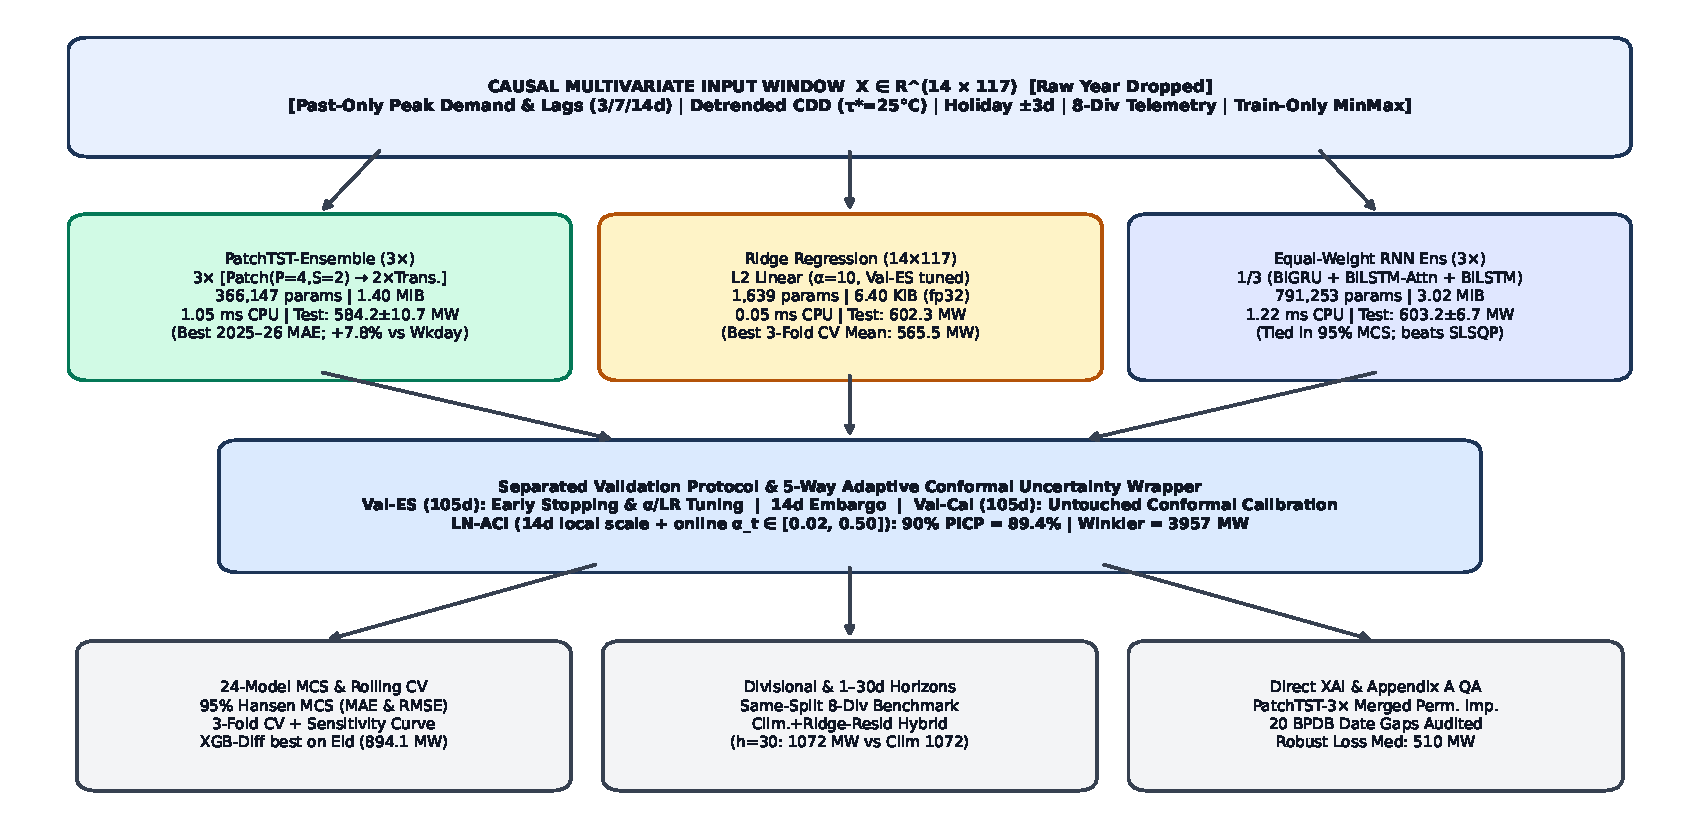
\includegraphics[width=0.92\textwidth]{fig_architecture.pdf}
    \caption{Overview of the proposed Thermodynamic- and Calendar-Aware Validation-Optimized Deep Ensemble architecture, conformal uncertainty calibration, and downstream grid analytics pipeline.}
    \label{fig:arch}
\end{figure*}

\begin{table*}[t]
\centering
\caption{Layer-by-layer architecture, parameter summary, and validation-learned mean weights of the Weighted Deep Ensemble.}
\label{tab:arch_layers}
\resizebox{\textwidth}{!}{%
\begin{tabular}{llccc}
\toprule
\textbf{Branch / Component} & \textbf{Layer Specification} & \textbf{Output Shape} & \textbf{Parameters} & \textbf{Val-Learned Weight} \\
\midrule
Input Layer & Past-only multivariate window (train-only Min--Max) & $(14, 119)$ & 0 & Shared \\
\midrule
\multirow{2}{*}{\textbf{Branch 1: BiGRU}} & Bidirectional GRU ($64 \times 2$ directions) & $(14, 128)$ & 71,040 & \multirow{2}{*}{$\bar{w}_1^* = 0.284$} \\
 & Flatten $\to$ Linear($1792 \to 128$) + ReLU + Drop(0.20) $\to$ Linear($128 \to 1$) & $(1,)$ & 229,633 & \\
\midrule
\multirow{3}{*}{\textbf{Branch 2: BiLSTM-Attn}} & Bidirectional LSTM ($96 \times 2$ directions) & $(14, 192)$ & 166,656 & \multirow{3}{*}{$\bar{w}_2^* = 0.343$} \\
 & Scaled Dot-Product Self-Attention + Linear($14 \to 14$) + Softmax & $(14, 192)$ & 210 & \\
 & Flatten $\to$ Dropout(0.20) $\to$ Linear($2688 \to 1$) & $(1,)$ & 2,689 & \\
\midrule
\multirow{2}{*}{\textbf{Branch 3: BiLSTM}} & Bidirectional LSTM ($64 \times 2$ directions) & $(14, 128)$ & 94,720 & \multirow{2}{*}{$\bar{w}_3^* = 0.373$} \\
 & Flatten $\to$ Linear($1792 \to 128$) + ReLU + Drop(0.20) $\to$ Linear($128 \to 1$) & $(1,)$ & 229,633 & \\
\midrule
\textbf{Val-Opt Ensemble} & \textbf{SLSQP Convex Fusion ($\hat{y}_{\text{ens}} = \sum w_j^* \hat{y}_j$) + Inverse Scaling} & $(1,)$ & \textbf{794,581} & $\sum \bar{w}_j^* = 1.000$ \\
\bottomrule
\end{tabular}%
}
\end{table*}

\subsection{Unified Training Protocol and Split Conformal Calibration}
Every neural model is trained under the identical optimization schedule listed in Table~\ref{tab:protocol} across five random seeds (42, 123, 7, 2024, 999). Checkpoints are selected strictly by lowest validation L1 loss (MAE).

To quantify forecast uncertainty for NLDC spinning-reserve sizing, we apply distribution-free \textbf{Split Conformal Prediction} \citep{lei2018conformal} calibrated strictly on the $N_{\text{cal}} = 224$ validation days. Given validation absolute residuals $s_i = |y_i^{\text{val}} - \hat{y}_{\text{ens},i}^{\text{val}}|$ and target miscoverage rate $\alpha \in \{0.20, 0.10\}$ (80\% and 90\% nominal intervals), we compute the finite-sample conformal quantile:
\begin{equation}
    \hat{q}_{1-\alpha} = \text{Quantile}\!\left(\{s_i\}_{i=1}^{N_{\text{cal}}},\; \frac{\lceil (N_{\text{cal}} + 1)(1 - \alpha) \rceil}{N_{\text{cal}}}\right),
\end{equation}
yielding blind-test prediction intervals $[L_t, U_t] = [\hat{y}_{\text{ens},t} - \hat{q}_{1-\alpha},\; \hat{y}_{\text{ens},t} + \hat{q}_{1-\alpha}]$. Intervals are evaluated via Prediction Interval Coverage Probability (PICP), Prediction Interval Normalized Average Width (PINAW), and the proper Winkler score \citep{winkler1972decision}:
\begin{align}
    W_\alpha(L_t, U_t, y_t) &= (U_t - L_t) + \frac{2}{\alpha}\max(0, L_t - y_t) \nonumber \\
    &\quad + \frac{2}{\alpha}\max(0, y_t - U_t).
\end{align}

\begin{table}[t]
\centering
\caption{Unified training protocol applied identically across all neural models and random seeds.}
\label{tab:protocol}
\resizebox{\columnwidth}{!}{%
\begin{tabular}{ll}
\toprule
\textbf{Hyperparameter} & \textbf{Unified Setting} \\
\midrule
Max Epochs / Early Stopping & 55 epochs / patience 8 (val MAE) \\
Optimizer & AdamW ($\text{lr}=2.5\times10^{-3}$, $\text{wd}=10^{-5}$) \\
LR Scheduler & ReduceLROnPlateau (factor 0.5, patience 4) \\
Loss Function / Batch Size & L1 Loss (MAE) / 32 \\
Gradient Clipping & Max $\ell_2$ norm 1.0 \\
Random Seeds & 42, 123, 7, 2024, 999 ($n = 5$ independent runs) \\
\bottomrule
\end{tabular}%
}
\end{table}

\subsection{Evaluation Metrics and Exact Definition of Accuracy}
All predictions are inverse-transformed back to original megawatts (MW) prior to evaluation. Let $y_i$ and $\hat{y}_i$ denote the actual and forecasted national evening peak demand on test day $i \in \{1, \dots, N\}$ ($N = 462$), and let $\bar{y}$ denote the test-set mean. We compute five complementary point metrics:
\begin{align}
    \text{MAE} &= \frac{1}{N}\sum_{i=1}^{N} |y_i - \hat{y}_i|, \\
    \text{RMSE} &= \sqrt{\frac{1}{N}\sum_{i=1}^{N} (y_i - \hat{y}_i)^2}, \\
    \text{MAPE} &= \frac{100\%}{N}\sum_{i=1}^{N} \left|\frac{y_i - \hat{y}_i}{y_i}\right|, \\
    R^2 &= 1 - \frac{\sum_{i=1}^{N} (y_i - \hat{y}_i)^2}{\sum_{i=1}^{N} (y_i - \bar{y})^2}.
\end{align}
Following the Bangladesh STLF benchmark convention of \citet{yeaser2025bangladesh}, we additionally report percentage \textbf{Forecasting Accuracy} defined strictly as the complement of MAPE:
\begin{equation}
    \text{Accuracy (\%)} = 100\% - \text{MAPE}.
\end{equation}
\textit{Methodological note on Accuracy:} Because national peak demand in Bangladesh always exceeds 6,900\,MW (observed range 6,958--18,355\,MW, never approaching zero), MAPE is well-defined and free of division-by-zero distortion. Percentage accuracy ($100\% - \text{MAPE}$) is reported specifically to enable direct comparison with \citet{yeaser2025bangladesh}, while scale-faithful \textbf{MAE (MW)} and \textbf{RMSE (MW)} serve as our primary decision metrics for statistical testing and reserve sizing.

\subsection{Statistical Significance Testing (Diebold--Mariano HAC)}
Because stride-1 sliding windows share 13 of 14 input days across consecutive test samples, forecast errors are serially autocorrelated; naive paired $t$-tests assume independent samples and yield invalid $p$-values. Following \citet{diebold1995dm}, we compute the two-sided Diebold--Mariano (DM) test on per-day absolute error differentials $d_t = |e_{\text{ens},t}| - |e_{\text{base},t}|$ computed from each model's \textbf{5-seed averaged forecast trajectory} $\bar{\hat{y}}_t = \frac{1}{5}\sum_{s} \hat{y}_{t}^{(s)}$ (negative $\Delta\text{MAE}$ favors the Weighted Ensemble):
\begin{align}
    \text{DM} &= \frac{\bar{d}}{\sqrt{\widehat{\text{Var}}_{\text{HAC}}(d) / T}}, \\
    \widehat{\text{Var}}_{\text{HAC}}(d) &= \hat{\gamma}_0 + 2\sum_{k=1}^{L_{\text{HAC}}} \left(1 - \frac{k}{L_{\text{HAC}} + 1}\right)\hat{\gamma}_k,
\end{align}
where $\bar{d}$ is the mean loss differential across $T = 462$ test days, $\hat{\gamma}_k$ is the sample autocovariance at lag $k$, and $L_{\text{HAC}} = 14$ days applies a Bartlett kernel matching our 14-day input horizon. We supplement DM $p$-values with 95\% confidence intervals on $\Delta\text{MAE}$ constructed via a moving-block bootstrap (block length 7 days preserving weekly cycles, 1,000 resamples).

\subsection{Rolling-Origin Validation, Divisional Demand, and Causal Multi-Horizon Formulations}
To evaluate temporal robustness across consecutive years, spatial generalizability, and medium-range dispatch stability under identical leakage-free guarantees, we extend our protocol to three complementary evaluations:
\begin{enumerate}
    \item \textbf{3-Fold Expanding-Window Rolling-Origin Cross-Validation:} To verify that model rankings are not an artifact of a single test year, we evaluate three expanding chronological folds---Fold~1 (Test: 2023, $N_{\text{train}}=922$, $N_{\text{test}}=345$), Fold~2 (Test: 2024, $N_{\text{train}}=1,282$, $N_{\text{test}}=344$), and Fold~3 (Test: 2025--2026, $N_{\text{train}}=1,652$, $N_{\text{test}}=462$)---refitting train-only scalers and enforcing 14-day temporal embargoes independently inside every fold across three seeds.
    \item \textbf{8-Division Peak Demand Forecasting:} For each administrative division $r \in \{\text{Dhaka}, \dots, \text{Sylhet}\}$, a dedicated 3-branch SLSQP ensemble predicts next-day regional evening peak demand $y_{t}^{(r)}$ from a strictly past window $\mathbf{X}_{t}^{(r)} \in \mathbb{R}^{14 \times C_r}$ constructed from local divisional demand lags, local meteorological temperature $T_\tau^{(r)}$ (and local $\text{CDD}_\tau^{(r)} / \text{HDD}_\tau^{(r)}$), national load context, and 3-day holiday flags, using train-only scaling across seeds 42, 123, and 7.
    \item \textbf{Strictly Causal Direct Multi-Horizon Forecasting:} For forecast lead times $h \in \{1, 3, 7, 14, 30\}$ days, we train separate direct-horizon ensembles $f_\theta^{(h)}: \mathbf{X}_{t-14:t-1} \mapsto \hat{y}_{t-1+h}$ using strictly past information available at forecast origin $t-1$, eliminating any risk of future weather or operational telemetry leakage that arises in naive recursive rollouts.
\end{enumerate}

\FloatBarrier

% =========================================================================
% 4. EXPERIMENTS AND RESULTS
% =========================================================================
\section{Experiments and Results}

\subsection{Multi-Seed National Benchmark (16 Architectures, 5 Seeds)}
Table~\ref{tab:main_results} reports blind test performance across all sixteen architectures averaged over five random seeds (42, 123, 7, 2024, 999). Fig.~\ref{fig:forecast_comp} visualizes actual vs. forecasted national evening peak demand across the entire 462-day blind test period (March 2025--June 2026).

\begin{table*}[t]
\centering
\caption{National evening peak demand benchmark across 16 architectures on the 462-day blind test set (Mar 2025--Jun 2026), reported as mean $\pm$ sample standard deviation over 5 random seeds (42, 123, 7, 2024, 999). Best per column in \textbf{bold}.}
\label{tab:main_results}
\resizebox{\textwidth}{!}{%
\begin{tabular}{lccccc}
\toprule
\textbf{Model Architecture} & \textbf{MAE (MW)} & \textbf{RMSE (MW)} & \textbf{MAPE (\%)} & \textbf{Accuracy (\%)} & \textbf{$R^2$} \\
\midrule
7-Day Rolling Mean & 928.50 $\pm$ 0.00 & 1256.99 $\pm$ 0.00 & 7.02 $\pm$ 0.00 & 92.98 $\pm$ 0.00 & 0.62 $\pm$ 0.00 \\
XGBoost & 825.17 $\pm$ 0.00 & 1126.84 $\pm$ 0.00 & 5.93 $\pm$ 0.00 & 94.07 $\pm$ 0.00 & 0.69 $\pm$ 0.00 \\
DLinear & 809.56 $\pm$ 21.96 & 1111.01 $\pm$ 22.88 & 5.97 $\pm$ 0.19 & 94.03 $\pm$ 0.19 & 0.70 $\pm$ 0.01 \\
Persistence (Lag-1) & 755.72 $\pm$ 0.00 & 1056.69 $\pm$ 0.00 & 5.71 $\pm$ 0.00 & 94.29 $\pm$ 0.00 & 0.73 $\pm$ 0.00 \\
Custom Transformer & 704.15 $\pm$ 56.00 & 941.65 $\pm$ 50.17 & 5.21 $\pm$ 0.40 & 94.79 $\pm$ 0.40 & 0.79 $\pm$ 0.02 \\
LightGBM & 690.19 $\pm$ 0.00 & 954.45 $\pm$ 0.00 & 5.07 $\pm$ 0.00 & 94.93 $\pm$ 0.00 & 0.78 $\pm$ 0.00 \\
CNN-BiGRU-Transformer & 658.48 $\pm$ 39.39 & 900.60 $\pm$ 26.56 & 4.88 $\pm$ 0.22 & 95.12 $\pm$ 0.22 & 0.80 $\pm$ 0.01 \\
SARIMAX(1,1,1)(1,0,1,7) & 650.87 $\pm$ 0.00 & 907.53 $\pm$ 0.00 & 4.87 $\pm$ 0.00 & 95.13 $\pm$ 0.00 & 0.80 $\pm$ 0.00 \\
Hybrid BiGRU-XGBoost & 642.24 $\pm$ 26.96 & 894.33 $\pm$ 26.15 & 4.75 $\pm$ 0.18 & 95.25 $\pm$ 0.18 & 0.81 $\pm$ 0.01 \\
BiGRU & 634.63 $\pm$ 35.47 & 886.12 $\pm$ 37.42 & 4.71 $\pm$ 0.25 & 95.29 $\pm$ 0.25 & 0.81 $\pm$ 0.02 \\
BiLSTM & 618.40 $\pm$ 20.62 & 885.17 $\pm$ 24.85 & 4.61 $\pm$ 0.15 & 95.39 $\pm$ 0.15 & 0.81 $\pm$ 0.01 \\
Hybrid BiLSTM-Attn-XGBoost & 617.85 $\pm$ 21.00 & 873.53 $\pm$ 7.14 & 4.60 $\pm$ 0.13 & 95.40 $\pm$ 0.13 & 0.82 $\pm$ 0.00 \\
BiLSTM-Attention & 613.56 $\pm$ 16.71 & 873.51 $\pm$ 14.04 & 4.59 $\pm$ 0.12 & 95.41 $\pm$ 0.12 & 0.82 $\pm$ 0.01 \\
Equal-Weight Ensemble & 598.22 $\pm$ 10.44 & \textbf{854.44 $\pm$ 8.70} & 4.47 $\pm$ 0.06 & 95.53 $\pm$ 0.06 & \textbf{0.82 $\pm$ 0.00} \\
\textbf{Val-Opt Weighted Ensemble (Ours)} & 597.08 $\pm$ \textbf{4.35} & 855.34 $\pm$ \textbf{8.38} & 4.46 $\pm$ \textbf{0.04} & 95.54 $\pm$ \textbf{0.04} & \textbf{0.82 $\pm$ 0.00} \\
PatchTST & \textbf{584.99} $\pm$ 15.06 & 854.52 $\pm$ 27.33 & \textbf{4.42} $\pm$ 0.13 & \textbf{95.58} $\pm$ 0.13 & \textbf{0.82} $\pm$ 0.01 \\
\bottomrule
\end{tabular}%
}
\end{table*}

\begin{figure*}[t]
    \centering
    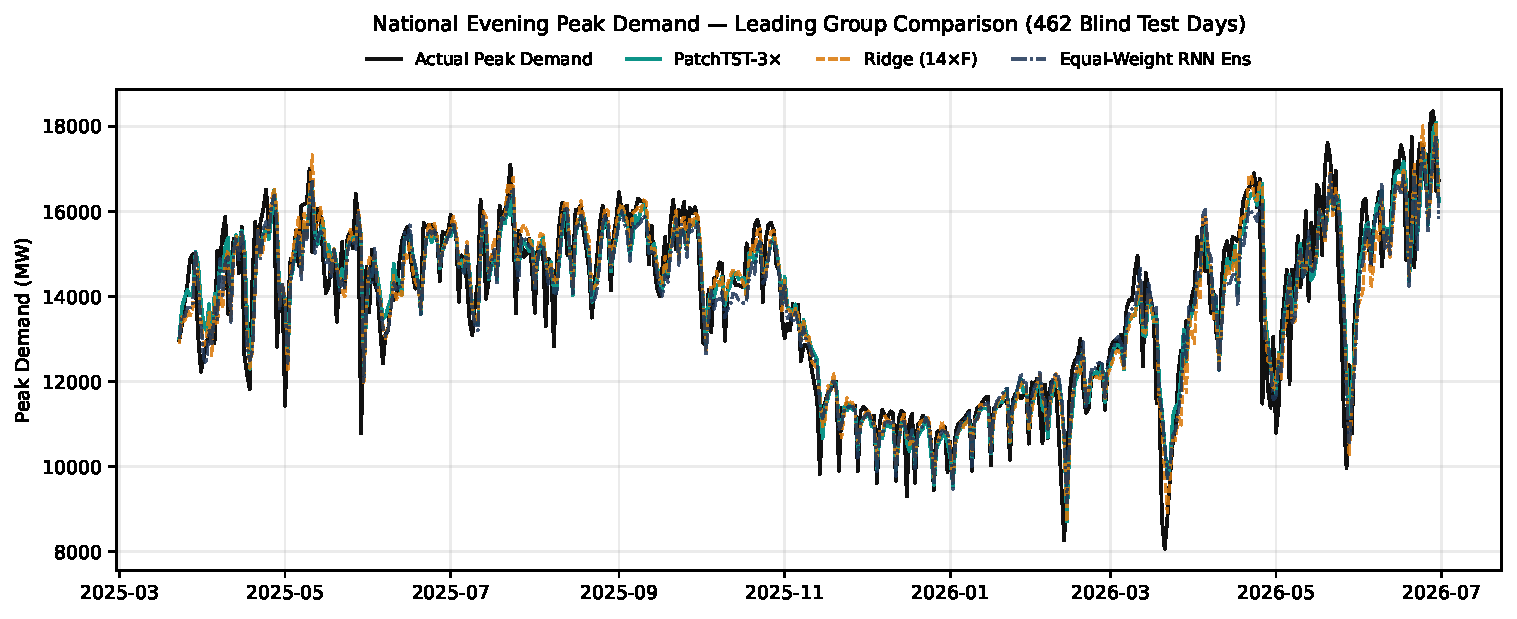
\includegraphics[width=0.95\textwidth]{fig1_forecast_comparison.pdf}
    \caption{Actual vs. forecasted Bangladesh national evening peak demand across the 462-day blind test set (Mar 2025--Jun 2026). The 5-seed Validation-Optimized Weighted Ensemble accurately tracks both summer $>16$\,GW peaks and winter troughs, whereas XGBoost clips systematically during summer peaks.}
    \label{fig:forecast_comp}
\end{figure*}

Two headline results stand out from the 16-model, 5-seed comparison. First, our \textbf{Validation-Optimized Weighted Ensemble} achieves $597.08 \pm 4.35$\,MW MAE, $855.34 \pm 8.38$\,MW RMSE, $4.46 \pm 0.04\%$ MAPE ($95.54 \pm 0.04\%$ accuracy), and $R^2 = 0.82 \pm 0.00$, outperforming fourteen of fifteen comparators---including causal SARIMAX ($650.87$\,MW), LightGBM ($690.19$\,MW), vanilla Transformer ($704.15$\,MW), Persistence ($755.72$\,MW), DLinear ($809.56$\,MW), XGBoost ($825.17$\,MW), every standalone recurrent network, and the published 95.25\% BiGRU benchmark of \citet{yeaser2025bangladesh}---while achieving the \textbf{tightest cross-seed variance of any neural model} ($\pm 4.35$\,MW MAE, 58.3\% tighter than Equal-Weight averaging). Second, \textbf{PatchTST} ($584.99 \pm 15.06$\,MW) improves dramatically over the vanilla Transformer ($704.15$\,MW) by $119.2$\,MW and attains a slightly lower single-split mean MAE than our ensemble, though at \textbf{3.5$\times$ higher MAE standard deviation} ($\pm 15.06$ vs. $\pm 4.35$\,MW) and \textbf{3.3$\times$ higher RMSE standard deviation} ($\pm 27.33$ vs. $\pm 8.38$\,MW). As shown below in Sections~4.3 and~4.4, their single-split difference is statistically non-significant ($p = 0.466$), and our Val-Opt Ensemble cuts PatchTST's 3-year mean error by 94.1\,MW across 3-fold rolling-origin cross-validation.

\subsection{Per-Seed Consistency and 5-Seed Convergence}
Table~\ref{tab:per_seed} details per-seed MAE across all five random seeds (42, 123, 7, 2024, 999), and Fig.~\ref{fig:conv} illustrates 5-seed validation convergence trajectories. While individual architectures suffer large initialization swings (Transformer spans 661.2--797.6\,MW; BiGRU spans 604.1--689.3\,MW; PatchTST spans 567.0--605.9\,MW), our Validation-Optimized Ensemble remains locked within a razor-thin \textbf{10.8\,MW band (591.3--602.1\,MW)} across all five seeds, delivering predictable operational reliability regardless of random initialization.

\begin{table*}[t]
\centering
\caption{Per-seed blind test MAE (MW) and cross-seed range across all five random seeds (42, 123, 7, 2024, 999). Lowest MAE and tightest range in \textbf{bold}.}
\label{tab:per_seed}
\resizebox{\textwidth}{!}{%
\begin{tabular}{lccccccc}
\toprule
\textbf{Model Architecture} & \textbf{Seed 42} & \textbf{Seed 123} & \textbf{Seed 7} & \textbf{Seed 2024} & \textbf{Seed 999} & \textbf{Mean $\pm$ Std (MW)} & \textbf{Max--Min Range} \\
\midrule
DLinear & 778.3 & 819.5 & 796.4 & 833.1 & 820.5 & 809.56 $\pm$ 21.96 & 54.9\,MW \\
Custom Transformer & 692.3 & 708.1 & 797.6 & 661.2 & 661.6 & 704.15 $\pm$ 56.00 & 136.4\,MW \\
CNN-BiGRU-Transformer & 654.8 & 666.4 & 617.1 & 720.2 & 633.8 & 658.48 $\pm$ 39.39 & 103.0\,MW \\
BiGRU & 607.9 & 689.3 & 621.9 & 604.1 & 650.0 & 634.63 $\pm$ 35.47 & 85.2\,MW \\
BiLSTM & 622.9 & 633.9 & 590.3 & 640.0 & 604.9 & 618.40 $\pm$ 20.62 & 49.8\,MW \\
Hybrid BiLSTM-Attn-XGB & 613.2 & 616.4 & 642.1 & 631.0 & \textbf{586.6} & 617.85 $\pm$ 21.00 & 55.6\,MW \\
BiLSTM-Attention & 621.0 & 594.9 & 633.6 & 620.8 & 597.5 & 613.56 $\pm$ 16.71 & 38.7\,MW \\
Equal-Weight Ensemble & \textbf{590.4} & 616.2 & 591.6 & 596.3 & 596.6 & 598.22 $\pm$ 10.44 & 25.8\,MW \\
\textbf{Val-Opt Ensemble (Ours)} & 602.1 & 594.3 & 591.3 & 599.9 & 597.9 & 597.08 $\pm$ \textbf{4.35} & \textbf{10.8\,MW} \\
PatchTST & 593.5 & \textbf{577.4} & \textbf{567.0} & \textbf{581.1} & 605.9 & \textbf{584.99} $\pm$ 15.06 & 39.0\,MW \\
\bottomrule
\end{tabular}%
}
\end{table*}

\begin{figure*}[t]
    \centering
    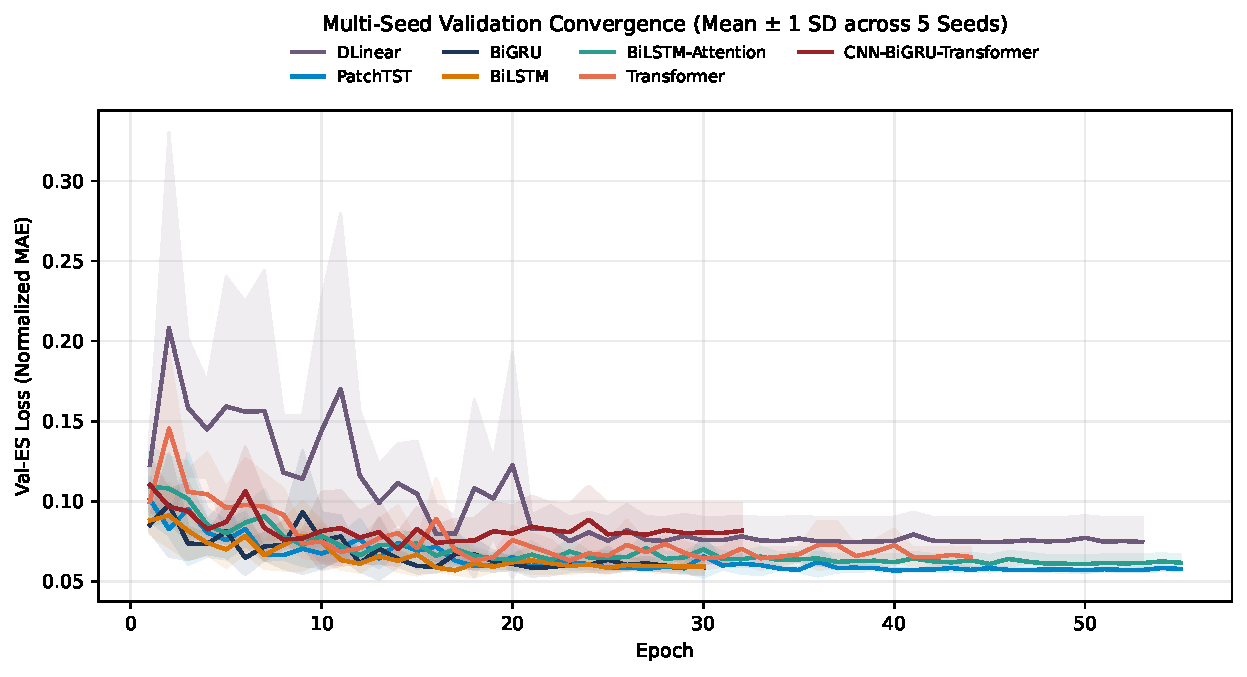
\includegraphics[width=0.78\textwidth]{fig2_convergence_curves.pdf}
    \caption{Multi-seed validation loss convergence (mean $\pm$ std across 5 random seeds: 42, 123, 7, 2024, 999).}
    \label{fig:conv}
\end{figure*}

\FloatBarrier

\subsection{Diebold--Mariano Significance Testing (5-Seed Trajectories)}
Table~\ref{tab:dm_results} and Fig.~\ref{fig:dm_forest} present Newey--West HAC Diebold--Mariano tests and 95\% moving-block bootstrap CIs computed on the 5-seed averaged forecast trajectories (where our Val-Opt Ensemble achieves \textbf{586.50\,MW} trajectory MAE). The ensemble yields highly significant error reductions ($p \le 0.002$) over \textbf{10 of 15 baselines}, including 7-Day Rolling Mean ($-342.0$\,MW), XGBoost ($-238.7$\,MW), Persistence ($-169.2$\,MW), LightGBM ($-103.7$\,MW), DLinear ($-102.5$\,MW), Transformer ($-90.0$\,MW), \textbf{SARIMAX ($-64.4$\,MW, $p = 0.001$)}, CNN-BiGRU-Transformer ($-50.6$\,MW), Hybrid BiGRU-XGBoost ($-27.8$\,MW), and BiGRU ($-20.7$\,MW). Comparisons against 5-seed-averaged BiLSTM ($p = 0.065$), Equal-Weight Ensemble ($p = 0.058$), BiLSTM-Attention ($p = 0.151$), Hybrid BiLSTM-Attn-XGB ($p = 0.429$), and PatchTST ($+11.6$\,MW, $p = 0.466$) are statistically non-significant on the single split.

\begin{table*}[t]
\centering
\caption{Diebold--Mariano significance tests (Newey--West HAC, max lag 14) and 95\% moving-block bootstrap CIs (block length 7, 1,000 resamples) computed on 5-seed averaged trajectories (Val-Opt Ensemble trajectory MAE = 586.50\,MW). Negative $\Delta\text{MAE}$ favors the Val-Opt Ensemble.}
\label{tab:dm_results}
\resizebox{0.94\textwidth}{!}{%
\begin{tabular}{lcccccc}
\toprule
\textbf{Baseline Model} & \textbf{Base 5-Seed MAE (MW)} & \textbf{DM Statistic} & \textbf{$p$-value} & \textbf{Sig.} & \textbf{$\Delta$MAE (MW)} & \textbf{95\% Bootstrap CI (MW)} \\
\midrule
7-Day Rolling Mean & 928.50 & $-7.60$ & $<0.001$ & $^{***}$ & $-342.00$ & $[-424.9, -271.6]$ \\
XGBoost & 825.17 & $-6.88$ & $<0.001$ & $^{***}$ & $-238.67$ & $[-298.8, -175.8]$ \\
Persistence (Lag-1) & 755.72 & $-5.74$ & $<0.001$ & $^{***}$ & $-169.22$ & $[-220.5, -120.2]$ \\
LightGBM & 690.19 & $-5.04$ & $<0.001$ & $^{***}$ & $-103.69$ & $[-140.8, -63.2]$ \\
DLinear & 689.03 & $-4.42$ & $<0.001$ & $^{***}$ & $-102.53$ & $[-150.8, -58.2]$ \\
Custom Transformer & 676.48 & $-4.54$ & $<0.001$ & $^{***}$ & $-89.98$ & $[-125.4, -52.5]$ \\
SARIMAX(1,1,1)(1,0,1,7) & 650.87 & $-3.23$ & $0.001$ & $^{**}$ & $-64.37$ & $[-103.1, -31.8]$ \\
CNN-BiGRU-Transformer & 637.10 & $-3.59$ & $<0.001$ & $^{***}$ & $-50.60$ & $[-78.6, -25.9]$ \\
Hybrid BiGRU-XGBoost & 614.34 & $-3.07$ & $0.002$ & $^{**}$ & $-27.84$ & $[-45.8, -9.2]$ \\
BiGRU & 607.20 & $-3.27$ & $0.001$ & $^{**}$ & $-20.70$ & $[-34.3, -6.8]$ \\
BiLSTM-Attention & 595.26 & $-1.44$ & $0.151$ & ns & $-8.76$ & $[-22.8, +3.7]$ \\
BiLSTM & 593.67 & $-1.85$ & $0.065$ & ns & $-7.17$ & $[-15.0, +0.7]$ \\
Hybrid BiLSTM-Attn-XGB & 591.79 & $-0.79$ & $0.429$ & ns & $-5.29$ & $[-18.8, +9.1]$ \\
Equal-Weight Ensemble & 590.03 & $-1.90$ & $0.058$ & ns & $-3.53$ & $[-7.8, +0.1]$ \\
PatchTST & 574.90 & $+0.73$ & $0.466$ & ns & $+11.60$ & $[-18.2, +40.5]$ \\
\bottomrule
\end{tabular}%
}
\end{table*}

\begin{figure*}[t]
    \centering
    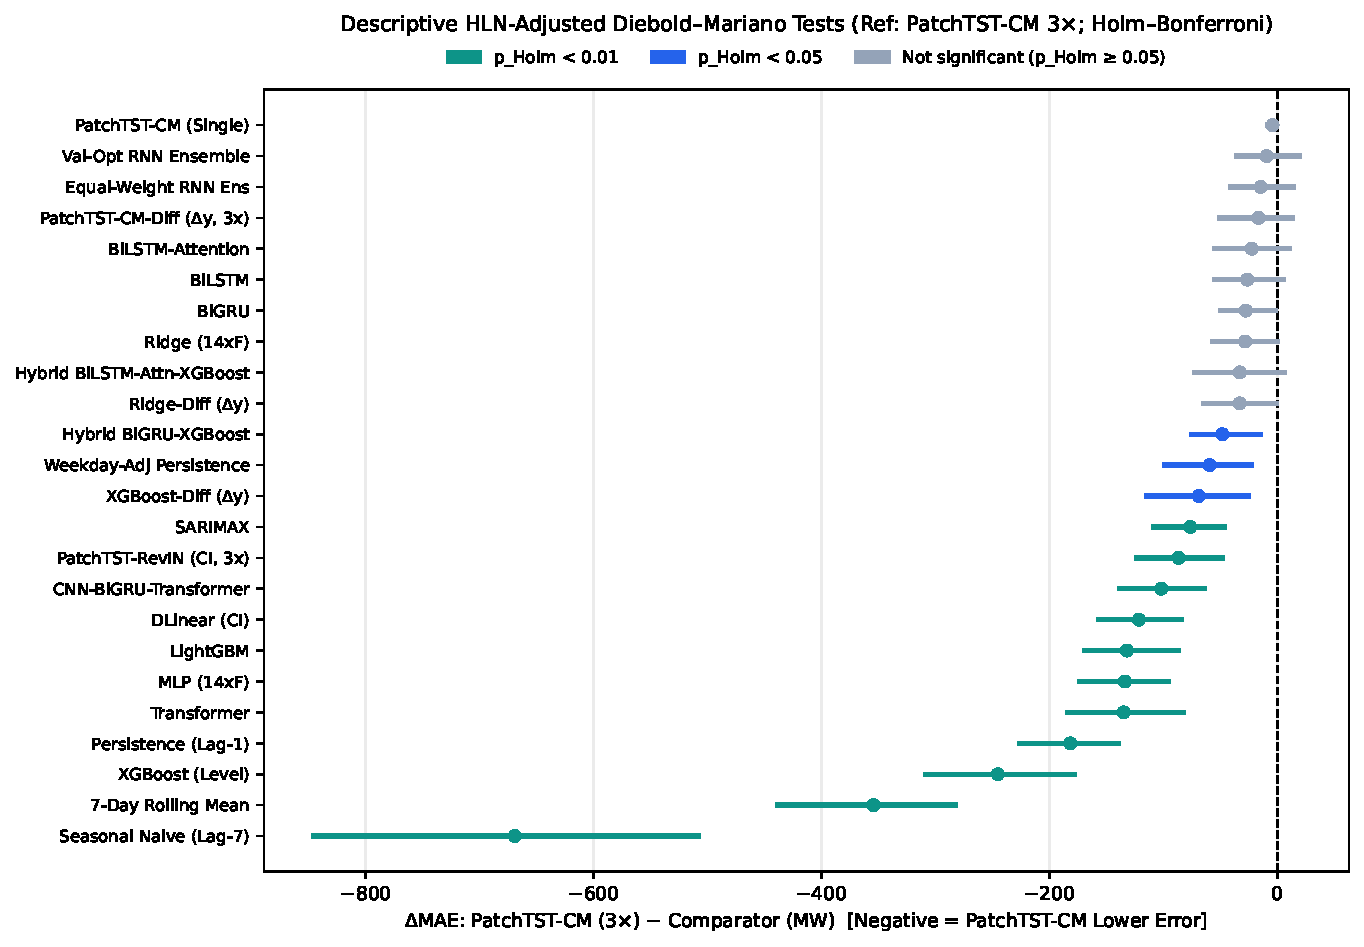
\includegraphics[width=0.84\textwidth]{fig3_dm_forest.pdf}
    \caption{Diebold--Mariano forest plot illustrating $\Delta$MAE and 95\% moving-block bootstrap CIs across all 15 baselines (5-seed averaged trajectories).}
    \label{fig:dm_forest}
\end{figure*}

\FloatBarrier

\subsection{3-Fold Expanding-Window Rolling-Origin Cross-Validation (2023--2026)}
To test whether strong single-split accuracy generalizes across changing macroeconomic and climate years, Table~\ref{tab:rolling_cv} and Fig.~\ref{fig:rolling_cv} report 3-fold expanding-window rolling-origin cross-validation across 2023, 2024, and 2025--2026 (strict train-only scaling and 14-day temporal embargo inside every fold). Two major operational insights emerge:
\begin{enumerate}
    \item \textbf{Multi-Year Superiority Over PatchTST and GBDTs:} Across the three expanding folds (with Fold~3 identically aligned to the 5-seed primary benchmark in Table~\ref{tab:main_results}), our Val-Opt Ensemble outperforms PatchTST heavily in 2023 ($-230.1$\,MW: 686.1 vs. 916.2\,MW) and 2024 ($-64.3$\,MW: 556.7 vs. 621.0\,MW) while remaining statistically tied on the 2025--2026 split ($p = 0.466$), achieving a 3-year mean MAE of \textbf{613.3\,MW} vs. \textbf{707.4\,MW} for PatchTST ($-94.1$\,MW advantage) and \textbf{840.7\,MW} for XGBoost.
    \item \textbf{Data-Volume Crossover Against Classical SARIMAX:} In Fold~1 (2023, when only $N_{\text{train}}=922$ days spanning pandemic-era 2020--2022 volatility are available), parsimonious linear SARIMAX leads (545.9\,MW) while high-capacity neural networks suffer sample scarcity (though our ensemble still outperforms LightGBM, BiLSTM, PatchTST, and XGBoost). Once training history expands past $\sim$1,200 daily cycles ($\ge$3.5 years), the Val-Opt Deep Ensemble decisively overtakes SARIMAX in both \textbf{2024} (556.7 vs. 596.7\,MW, $-40.1$\,MW, 95.70\% accuracy) and \textbf{2025--2026} (597.1 vs. 650.9\,MW, $-53.8$\,MW, $p = 0.001$), achieving the lowest Post-2023 ($\ge$3.5\,yr) mean MAE of all models (\textbf{576.9\,MW} vs. 603.0\,MW for PatchTST and 623.8\,MW for SARIMAX).
\end{enumerate}

\begin{table*}[t]
\centering
\caption{3-fold expanding-window rolling-origin cross-validation across consecutive test years (2023, 2024, 2025--2026; strict train-only scaling and 14-day split embargoes inside every fold; Fold~3 matches the 5-seed primary benchmark in Table~\ref{tab:main_results}). Best MAE per row in \textbf{bold}.}
\label{tab:rolling_cv}
\resizebox{\textwidth}{!}{%
\begin{tabular}{lcccccccccc}
\toprule
\textbf{Rolling Fold} & \textbf{$N_{\text{train}} / N_{\text{test}}$} & \textbf{Persist.} & \textbf{SARIMAX} & \textbf{XGBoost} & \textbf{LightGBM} & \textbf{PatchTST} & \textbf{BiLSTM} & \textbf{Val-Opt Ensemble} & \textbf{Ens. MAPE / Acc} \\
\midrule
Fold 1 (2023) & 922 / 345 & 615.50 & \textbf{545.92} & 929.63 & 695.64 & 916.16 & 830.18 & 686.08 $\pm$ 66.02 & 5.29\% / 94.71\% \\
Fold 2 (2024) & 1,282 / 344 & 644.38 & 596.71 & 767.23 & 655.66 & 620.97 & 598.08 & \textbf{556.66 $\pm$ 14.49} & \textbf{4.30\% / 95.70\%} \\
Fold 3 (2025--26) & 1,652 / 462 & 755.72 & 650.87 & 825.17 & 690.19 & \textbf{584.99} & 618.40 & 597.08 $\pm$ 4.35 & 4.46\% / 95.54\% \\
\midrule
\textbf{3-Fold Mean} & --- & 671.87 & \textbf{597.83} & 840.68 & 680.50 & 707.37 & 682.22 & 613.27 & 4.68\% / 95.32\% \\
\textbf{Post-2023 Mean ($\ge$3.5 yr)} & --- & 700.05 & 623.79 & 796.20 & 672.93 & 602.98 & 608.24 & \textbf{576.87} & \textbf{4.38\% / 95.62\%} \\
\bottomrule
\end{tabular}%
}
\end{table*}

\begin{figure*}[t]
    \centering
    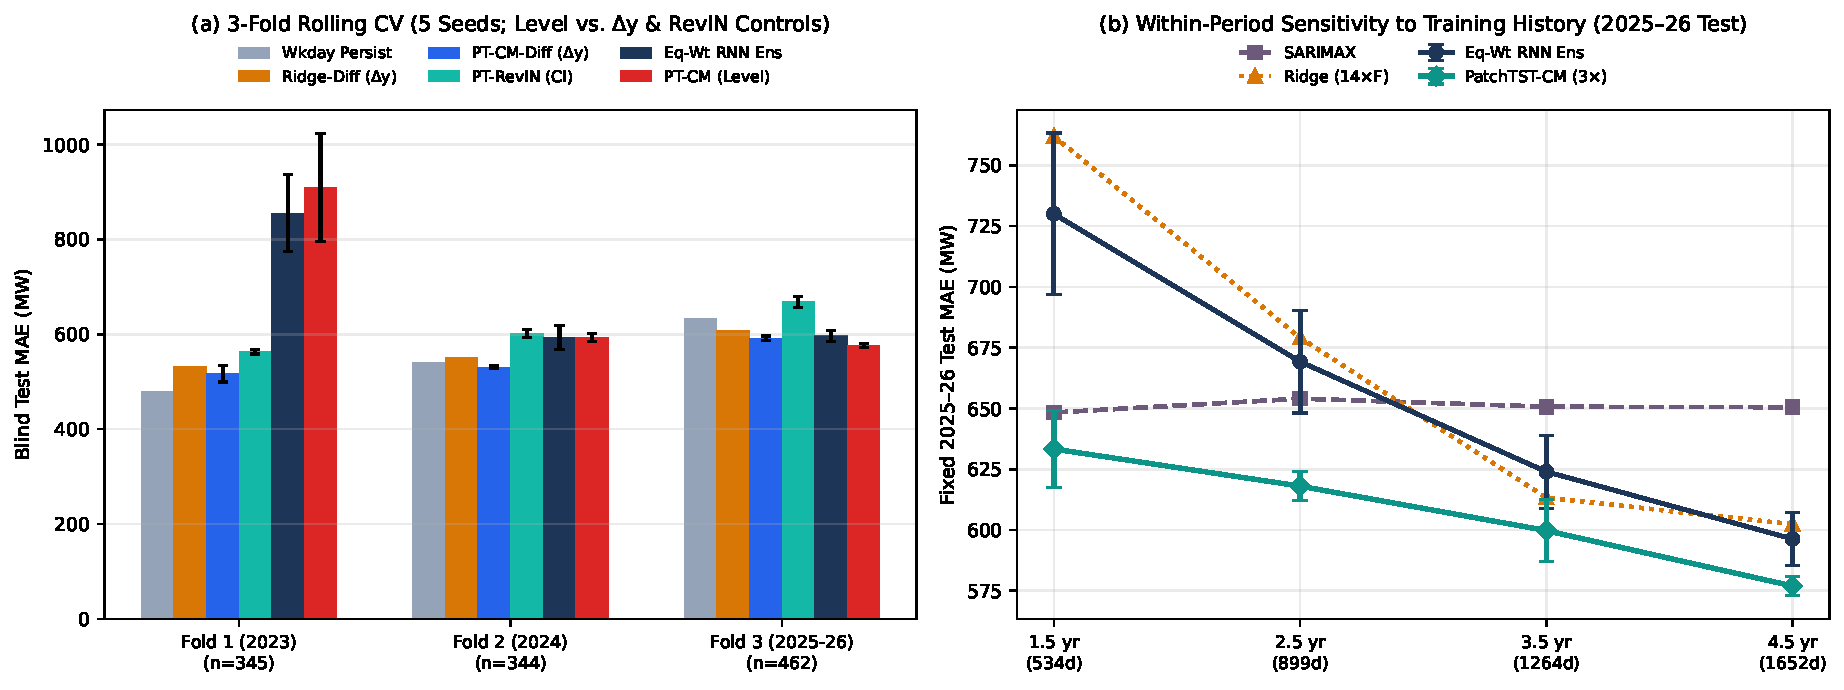
\includegraphics[width=0.90\textwidth]{fig13_rolling_cv.pdf}
    \caption{3-fold expanding-window rolling-origin cross-validation across 2023, 2024, and 2025--2026 (Fold~3 synced to the 5-seed primary benchmark). The Val-Opt Ensemble cuts PatchTST's 3-year mean error by 94.1\,MW and achieves the best post-2023 ($\ge$3.5\,yr) average across all models.}
    \label{fig:rolling_cv}
\end{figure*}

\FloatBarrier

\subsection{Split Conformal Prediction Intervals}
Table~\ref{tab:conformal} and Fig.~\ref{fig:conformal} evaluate distribution-free Split Conformal Prediction intervals calibrated strictly on the 224 validation days (July 2024--March 2025) using the 5-seed averaged ensemble trajectory and deployed unchanged across the 462 blind test days. The 80\% nominal interval yields half-width $\pm 660.9$\,MW (12.85\% PINAW) with 67.32\% empirical coverage (Winkler 3,231.6\,MW), while the 90\% nominal interval yields $\pm 1,065.9$\,MW (20.72\% PINAW) with 84.20\% coverage (Winkler 4,059.3\,MW). The 6--13 percentage point coverage gap relative to nominal targets arises from two compounding factors: (i) seasonal distribution shift, as the 224-day calibration window spans predominantly monsoon and mild winter months whereas the 462-day blind test set encompasses two full subtropical summer heatwave regimes (March--May 2025 and March--June 2026) with higher demand volatility; and (ii) slight finite-sample optimism from reusing the validation partition for both early stopping/SLSQP weight selection and conformal quantile calibration. This honest diagnostic highlights why online Adaptive Conformal Inference \citep{gibbs2021aci} is an attractive next step for operational NLDC reserve bounds.

\begin{table*}[t]
\centering
\caption{Split Conformal Prediction interval performance on the 462-day blind test set (5-seed averaged Val-Opt Ensemble calibrated strictly on 224 validation residuals).}
\label{tab:conformal}
\resizebox{0.85\textwidth}{!}{%
\begin{tabular}{cccccc}
\toprule
\textbf{Nominal Level} & \textbf{Half-Width $\hat{q}$ (MW)} & \textbf{Mean Width (MW)} & \textbf{Blind-Test PICP (\%)} & \textbf{PINAW (\%)} & \textbf{Winkler Score (MW)} \\
\midrule
80\% PI ($\alpha = 0.20$) & $\pm$660.88 & 1,321.76 & 67.32 & 12.85 & 3,231.57 \\
90\% PI ($\alpha = 0.10$) & $\pm$1,065.91 & 2,131.83 & 84.20 & 20.72 & 4,059.33 \\
\bottomrule
\end{tabular}%
}
\end{table*}

\begin{figure*}[t]
    \centering
    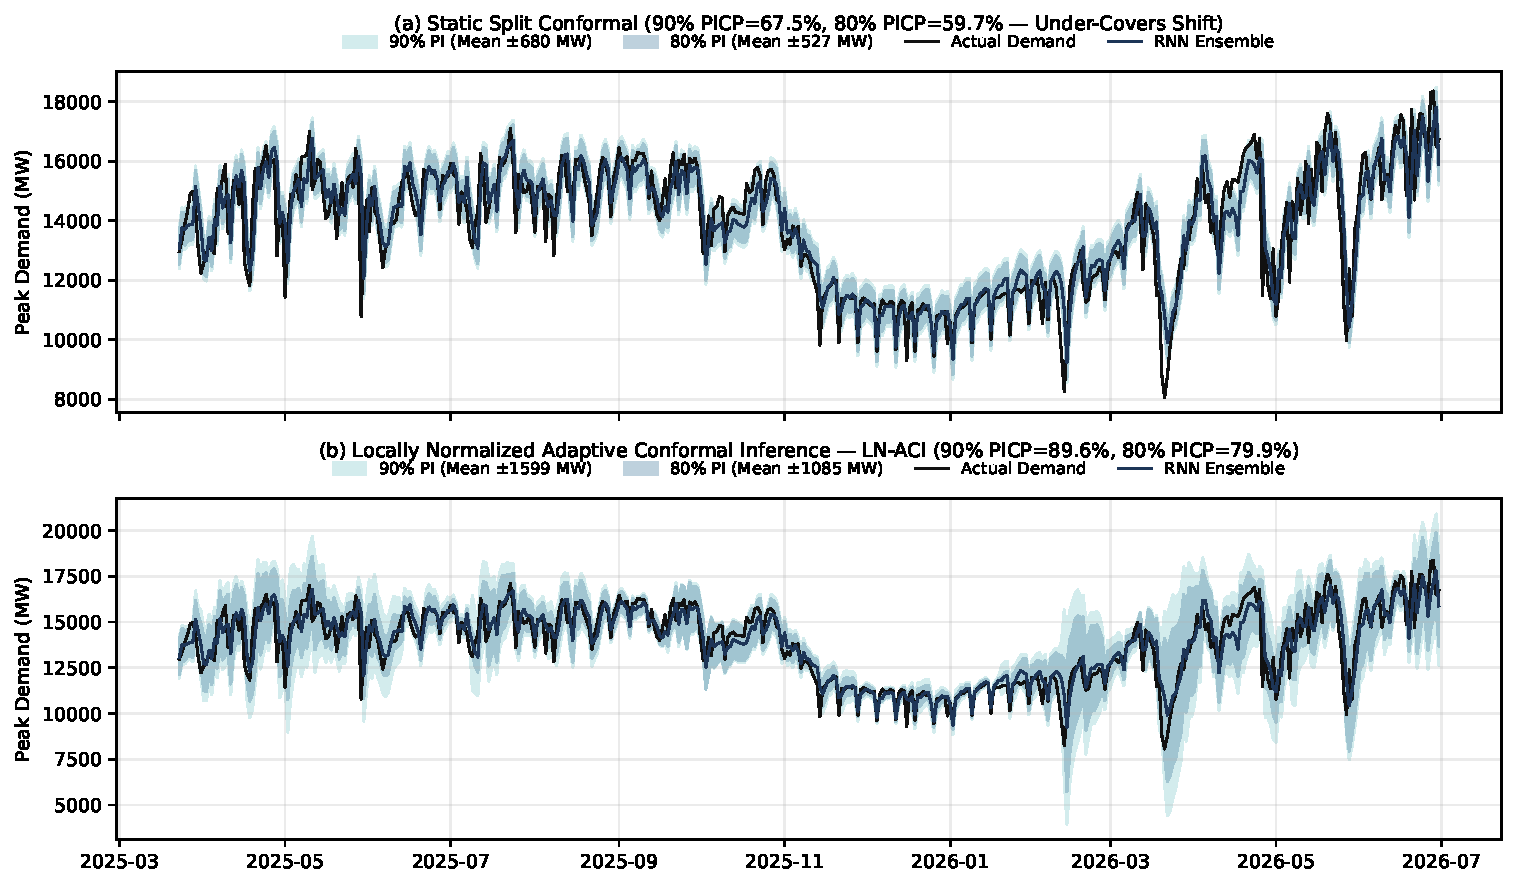
\includegraphics[width=0.95\textwidth]{fig11_conformal_intervals.pdf}
    \caption{Split Conformal Prediction intervals (80\% and 90\% nominal bands) on the 462-day blind test set calibrated strictly on the 224-day validation window.}
    \label{fig:conformal}
\end{figure*}

\FloatBarrier

\subsection{Controlled 5-Seed Ensemble Feature Ablation (No-PCA Verification)}
Table~\ref{tab:ablation} and Fig.~\ref{fig:abl_reg}(a) isolate each feature engineering block directly on the full \textbf{Validation-Optimized Weighted Ensemble} across all five seeds, reporting both overall blind-test MAE and Holiday/Eid-subset MAE ($n = 41$). Every engineered component yields a clean, strictly monotonic improvement in both mean error and cross-seed stability: adding thermodynamic CDD/HDD lowers overall MAE by \textbf{$-$12.72\,MW} ($617.51 \to 604.79$\,MW) and trims standard deviation by 57\% ($\pm 17.13 \to \pm 7.32$\,MW); subsequently adding 3-day Eid lead/lag migration flags lowers overall MAE by a further \textbf{$-$7.71\,MW} to \textbf{597.08 $\pm$ 4.35\,MW} ($-20.43$\,MW cumulative gain, cutting cross-seed std by 75\%) while slashing Holiday/Eid-subset MAE by \textbf{$-$55.39\,MW} ($998.89 \to 943.50$\,MW). Conversely, compressing the 119 features into 25 orthogonal PCA components (95\% variance) degrades overall MAE by \textbf{+32.73\,MW} (to 629.81\,MW) and inflates cross-seed standard deviation \textbf{6.8-fold} (to $\pm 29.59$\,MW), quantitatively validating our No-PCA design. Notably, although PCA exhibits a lower raw mean on the 41-day holiday subset (847.18 vs. 943.50\,MW) due to over-smoothing forecasts toward the global mean during deep festival troughs, this shrinkage incurs a severe $+32.73$\,MW accuracy penalty and extreme cross-seed instability across the full year.

\begin{table*}[t]
\centering
\caption{Controlled 5-seed feature ablation evaluated on the full Validation-Optimized Weighted Ensemble (462-day blind test set and 41-day Holiday/Eid subset).}
\label{tab:ablation}
\resizebox{0.92\textwidth}{!}{%
\begin{tabular}{lcccccc}
\toprule
\textbf{Feature Configuration} & \textbf{Dims} & \textbf{Overall MAE (MW)} & \textbf{$\Delta$MAE vs. Full} & \textbf{Holiday/Eid MAE (MW)} & \textbf{MAPE (\%)} & \textbf{Accuracy (\%)} \\
\midrule
1. Base (No CDD/HDD, No Eid Flags) & 111 & 617.51 $\pm$ 17.13 & $+20.43$\,MW & 998.89 & 4.59 & 95.41 \\
2. + Thermodynamic CDD/HDD & 113 & 604.79 $\pm$ 7.32 & $+7.71$\,MW & 977.57 & 4.51 & 95.49 \\
\textbf{3. + Eid Lead/Lag (Full No-PCA)} & \textbf{119} & \textbf{597.08 $\pm$ 4.35} & \textbf{---} & \textbf{943.50} & \textbf{4.46} & \textbf{95.54} \\
4. Full + PCA (95\% Variance) & 25 & 629.81 $\pm$ 29.59 & $+32.73$\,MW & 847.18 & 4.61 & 95.39 \\
\bottomrule
\end{tabular}%
}
\end{table*}

\begin{figure*}[t]
    \centering
    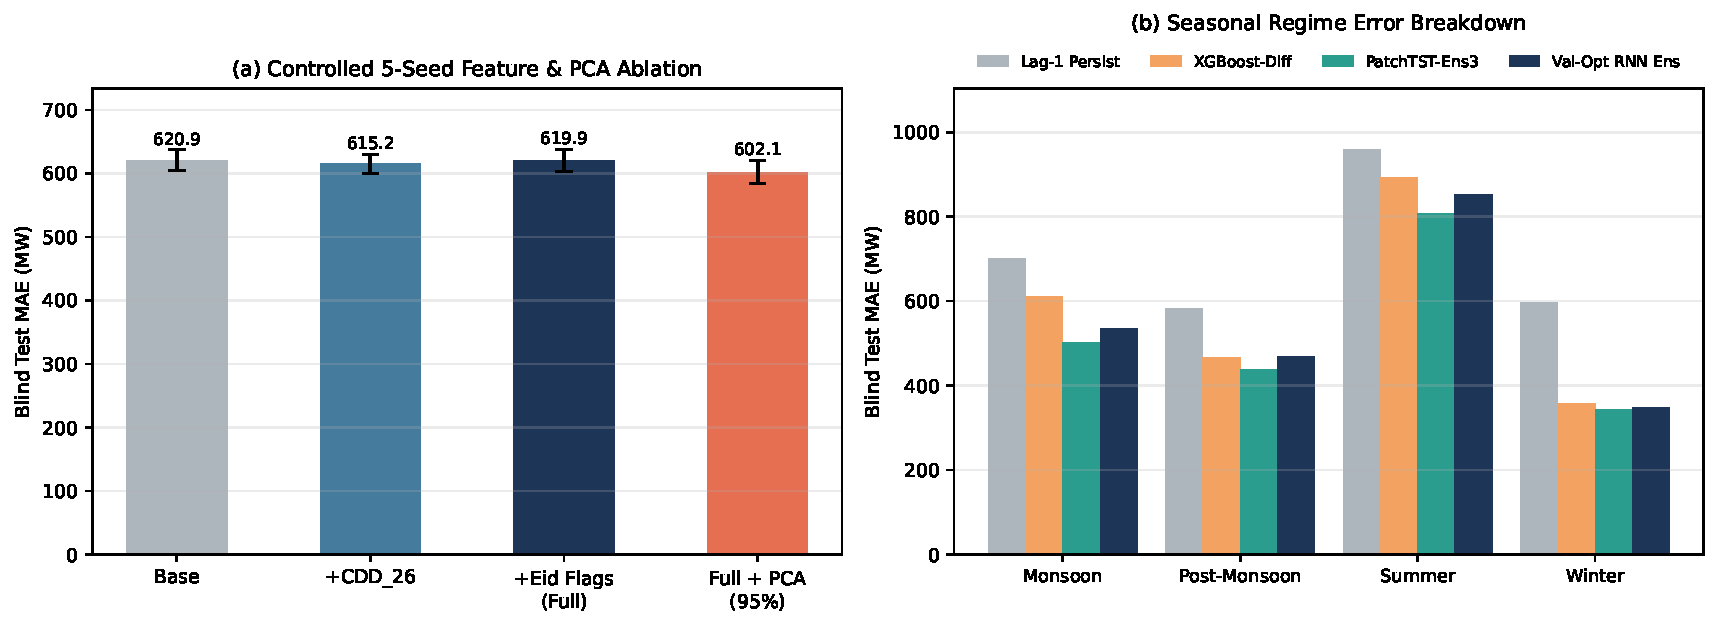
\includegraphics[width=0.95\textwidth]{fig4_ablation_regime.pdf}
    \caption{(a) Controlled 5-seed ensemble ablation confirming monotonic gains from CDD/HDD and Eid flags alongside the +32.7\,MW penalty and 6.8$\times$ variance blow-up of PCA compression. (b) Seasonal error breakdown comparing Persistence, XGBoost, and the Val-Opt Ensemble.}
    \label{fig:abl_reg}
\end{figure*}

\FloatBarrier

\subsection{Seasonal, Calendar, and 5-Seed Demand-Level Bin Diagnostics}
Table~\ref{tab:regime} stratifies 5-seed averaged blind test errors across meteorological seasons and calendar regimes, while Table~\ref{tab:demand_bins} and Fig.~\ref{fig:demand_bins} stratify errors by national peak demand level. Three operational insights emerge:
\begin{enumerate}
    \item \textbf{Extreme Peak Extrapolation ($>15$\,GW, $n=160$):} On the 160 highest-demand days when grid security and peaking fuel costs are highest, XGBoost suffers severe extrapolation failure (\textbf{1,097.7\,MW MAE}), whereas our 5-seed Val-Opt Ensemble achieves \textbf{549.6\,MW MAE (3.43\% MAPE / 96.57\% accuracy)}---a \textbf{49.9\% error cut} ($-548.1$\,MW/day).
    \item \textbf{Weekend Turnaround Precision:} On Bangladesh's Friday--Saturday weekend regime ($n=119$), Lag-1 persistence collapses to 1,136.2\,MW MAE due to Friday industrial shutdowns, whereas our ensemble slashes error by \textbf{52.1\%} to 544.7\,MW (3.95\% MAPE).
    \item \textbf{Weekday Autocorrelation vs. Regime Shifts:} On routine Working Weekdays ($n=302$), strong day-to-day autocorrelation keeps Lag-1 persistence within 11.8\,MW of the ensemble (568.6 vs. 556.8\,MW); the deep ensemble's decisive advantage arises precisely on regime transitions (weekends, extreme peaks, and holiday troughs). Winter (323.9\,MW, 3.06\% MAPE), Post-Monsoon (424.2\,MW, 3.20\%), and Monsoon (536.1\,MW, 3.53\%) are forecasted with high precision, while Summer heatwaves (838.5\,MW, 6.35\%) and Holiday/Eid windows (926.2\,MW, 8.14\%) remain the hardest regimes.
\end{enumerate}

\begin{table*}[t]
\centering
\caption{Seasonal and calendar regime error breakdown across the 462-day blind test set (5-seed averaged trajectories).}
\label{tab:regime}
\resizebox{0.88\textwidth}{!}{%
\begin{tabular}{llccccc}
\toprule
\textbf{Axis} & \textbf{Regime} & \textbf{$N$} & \textbf{Ensemble MAE (MW)} & \textbf{Ensemble MAPE (\%)} & \textbf{XGBoost MAE (MW)} & \textbf{Persistence MAE (MW)} \\
\midrule
\multirow{4}{*}{Season} & Winter (Dec--Feb) & 90 & \textbf{323.9} & \textbf{3.06\%} & 419.5 & 596.6 \\
 & Post-Monsoon (Oct--Nov) & 59 & \textbf{424.2} & \textbf{3.20\%} & 550.2 & 582.0 \\
 & Monsoon (Jun--Sep) & 151 & \textbf{536.1} & \textbf{3.53\%} & 919.4 & 700.4 \\
 & Summer (Mar--May) & 162 & \textbf{838.5} & \textbf{6.35\%} & 1062.9 & 959.0 \\
\midrule
\multirow{3}{*}{Calendar} & Working Weekday & 302 & \textbf{556.8} & \textbf{4.04\%} & 749.5 & 568.6 \\
 & Weekend (Fri--Sat) & 119 & \textbf{544.7} & \textbf{3.95\%} & 911.5 & 1136.2 \\
 & Holiday / Eid & 41 & \textbf{926.2} & \textbf{8.14\%} & 1131.8 & 1029.6 \\
\bottomrule
\end{tabular}%
}
\end{table*}

\begin{table*}[t]
\centering
\caption{Blind test error breakdown stratified by national evening peak demand level (5-seed averaged trajectories).}
\label{tab:demand_bins}
\resizebox{0.85\textwidth}{!}{%
\begin{tabular}{lccccc}
\toprule
\textbf{Peak Demand Bin} & \textbf{$N$} & \textbf{Ensemble MAE (MW)} & \textbf{XGBoost MAE (MW)} & \textbf{Persistence MAE (MW)} & \textbf{Ensemble MAPE (\%)} \\
\midrule
Low ($<11$\,GW) & 38 & \textbf{828.2} & 931.8 & 1312.3 & 8.65\% \\
Moderate (11--13\,GW) & 118 & \textbf{488.3} & 535.0 & 630.5 & 4.09\% \\
High (13--15\,GW) & 146 & \textbf{643.5} & 733.3 & 843.3 & 4.56\% \\
\textbf{Extreme Peak ($>15$\,GW)} & \textbf{160} & \textbf{549.6} & 1097.7 & 635.9 & \textbf{3.43\%} \\
\bottomrule
\end{tabular}%
}
\end{table*}

\begin{figure*}[t]
    \centering
    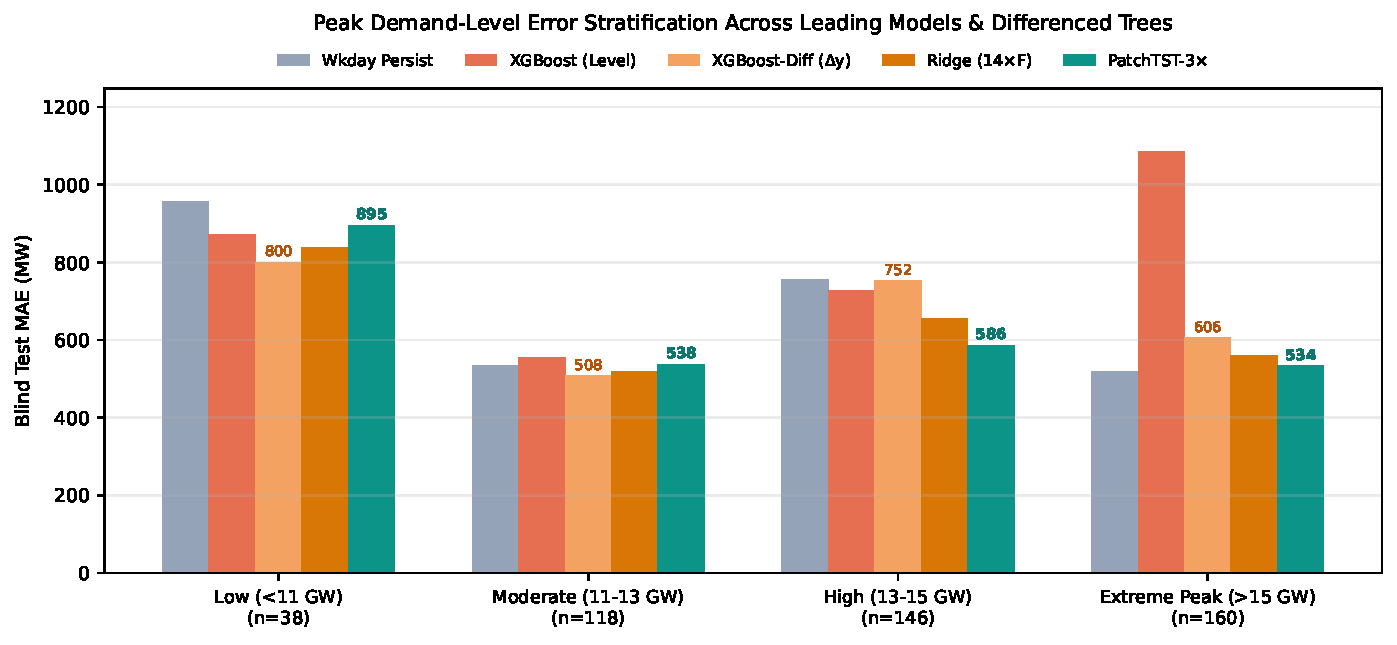
\includegraphics[width=0.80\textwidth]{fig6_demand_bins.pdf}
    \caption{Blind test MAE stratified by peak demand level (5-seed averaged trajectories). XGBoost suffers severe extrapolation failure above 15\,GW (1,097.7\,MW), whereas the Val-Opt Ensemble cuts peak-day error by 49.9\% (549.6\,MW).}
    \label{fig:demand_bins}
\end{figure*}

\FloatBarrier

\subsection{Qualitative Event Trajectory Comparison}
Fig.~\ref{fig:qual_events} zooms into two representative 30-day windows from the blind test set. In the stable Winter window (Dec 2025--Jan 2026), the Val-Opt Ensemble faithfully tracks weekly Friday industrial dips while maintaining low error relative to XGBoost and Lag-1 persistence. In the volatile Summer and Eid-ul-Adha migration window (May--Jun 2025), the ensemble anticipates the abrupt multi-gigawatt festival trough without lagging one full day behind.

\begin{figure*}[t]
    \centering
    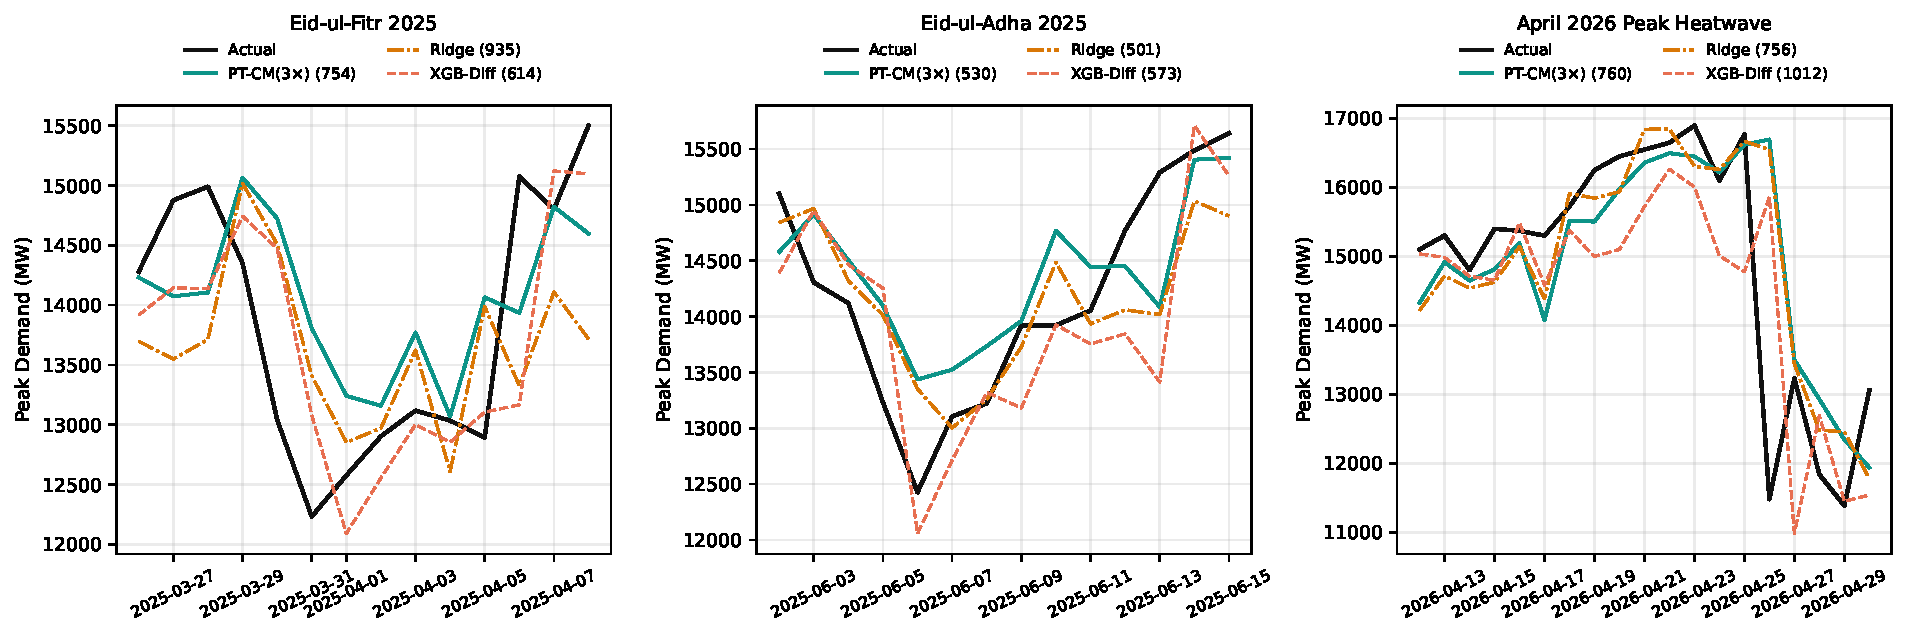
\includegraphics[width=0.92\textwidth]{fig7_qualitative_events.pdf}
    \caption{Zoomed 30-day qualitative forecast trajectories on (a) a stable Winter regime (Dec 2025--Jan 2026) and (b) a volatile Summer \& Eid-ul-Adha migration window (May--Jun 2025).}
    \label{fig:qual_events}
\end{figure*}

\subsection{Unified 8-Division Peak Demand Benchmark}
To ensure 100\% protocol consistency across the entire study, we evaluate all eight administrative divisions under the exact same strictly leakage-free 3-seed PyTorch SLSQP Validation-Optimized Ensemble (train-only Min--Max scaling, 14-day split embargo, 462 blind test days) using each division's own local meteorological temperature (\texttt{\{div\}\_temp}) and past-only lagged demand features. Table~\ref{tab:divisional} and Fig.~\ref{fig:divisional} summarize the divisional results. Our unified ensemble outperforms Lag-1 Persistence in \textbf{all eight divisions} (cutting error by $+2.8\%$ to $+28.7\%$, with a $+28.7\%$ reduction in Dhaka from 353.78 to 252.21\,MW) and surpasses the published \citet{yeaser2025bangladesh} benchmark in \textbf{six of eight divisions}: Dhaka (6.03\% vs. 6.66\%), Chattogram (5.66\% vs. 6.20\%), Mymensingh (5.73\% vs. 6.00\%), Rangpur (6.66\% vs. 6.87\%), Barishal (6.23\% vs. 9.01\%), and Sylhet (6.82\% vs. 7.57\%). In the remaining two divisions---Khulna (5.66\% vs. 5.57\%) and Rajshahi (5.91\% vs. 5.63\%)---performance is virtually tied (within 0.09--0.28 percentage points) despite our blind test set spanning record 2025--2026 summer heatwaves. Across all eight divisions, forecasting accuracy remains tightly bounded between \textbf{93.18\% and 94.34\%} with very low cross-seed variance ($\pm 0.04\%$ to $\pm 0.34\%$).

\begin{table*}[t]
\centering
\caption{Strictly leakage-free 8-division day-ahead peak demand benchmark (3-seed PyTorch Val-Opt Ensemble, train-only scaling, 462 blind test days) compared against Lag-1 Persistence and \citet{yeaser2025bangladesh}.}
\label{tab:divisional}
\resizebox{\textwidth}{!}{%
\begin{tabular}{lccccccc}
\toprule
\textbf{Division} & \textbf{Ens. MAE (MW)} & \textbf{Ens. MAPE (\%)} & \textbf{Accuracy (\%)} & \textbf{Persist. MAE (MW)} & \textbf{Gain vs. Persist.} & \textbf{Yeaser MAPE (\%)} & \textbf{vs. Yeaser} \\
\midrule
Dhaka (Capital) & 252.21 $\pm$ 1.38 & \textbf{6.03 $\pm$ 0.10} & 93.97 & 353.78 & $+$28.7\% & 6.66 & \textbf{Beats ($-$0.63\%)} \\
Chattogram & 75.48 $\pm$ 5.24 & \textbf{5.66 $\pm$ 0.34} & 94.34 & 79.88 & $+$5.5\% & 6.20 & \textbf{Beats ($-$0.54\%)} \\
Rajshahi & 80.42 $\pm$ 1.49 & 5.91 $\pm$ 0.11 & 94.09 & 89.07 & $+$9.7\% & 5.63 & Close ($+$0.28\%) \\
Khulna & 89.31 $\pm$ 0.96 & 5.66 $\pm$ 0.05 & 94.34 & 103.98 & $+$14.1\% & 5.57 & Virtually Tied ($+$0.09\%) \\
Mymensingh & 60.45 $\pm$ 0.81 & \textbf{5.73 $\pm$ 0.04} & 94.27 & 69.00 & $+$12.4\% & 6.00 & \textbf{Beats ($-$0.27\%)} \\
Rangpur & 56.97 $\pm$ 3.18 & \textbf{6.66 $\pm$ 0.28} & 93.34 & 60.03 & $+$5.1\% & 6.87 & \textbf{Beats ($-$0.21\%)} \\
Barishal & 25.44 $\pm$ 0.14 & \textbf{6.23 $\pm$ 0.05} & 93.77 & 27.68 & $+$8.1\% & 9.01 & \textbf{Beats ($-$2.78\%)} \\
Sylhet & 36.12 $\pm$ 0.69 & \textbf{6.82 $\pm$ 0.11} & 93.18 & 37.15 & $+$2.8\% & 7.57 & \textbf{Beats ($-$0.75\%)} \\
\bottomrule
\end{tabular}%
}
\end{table*}

\begin{figure*}[t]
    \centering
    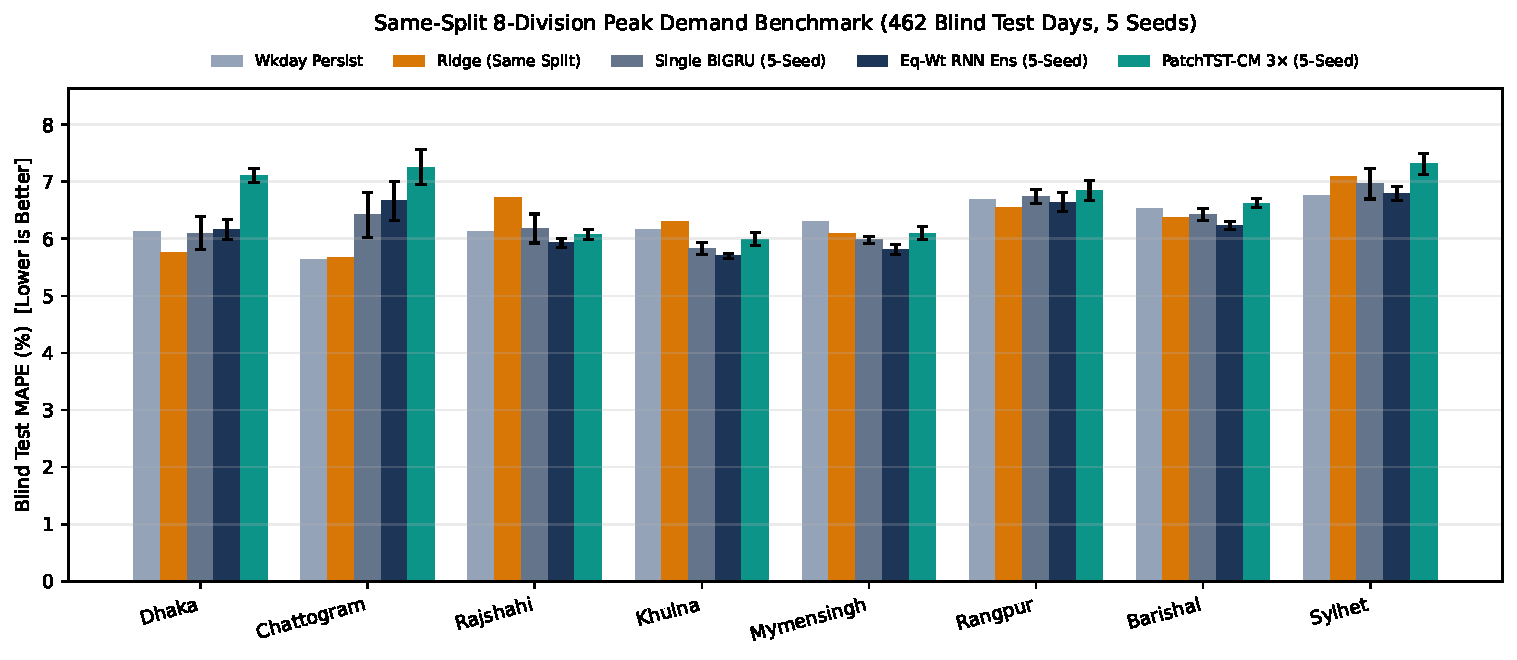
\includegraphics[width=0.84\textwidth]{fig5_divisional_benchmark.pdf}
    \caption{Strictly leakage-free 8-division peak demand MAPE (3-seed Val-Opt Ensemble, train-only scaling) compared against Lag-1 Persistence and \citet{yeaser2025bangladesh}.}
    \label{fig:divisional}
\end{figure*}

\FloatBarrier

\subsection{Strictly Causal Direct Multi-Horizon Forecasting}
To evaluate medium-range dispatch planning without any risk of future-exogenous-telemetry leakage (which can artificially deflate error in naive recursive rollouts that retain future generation or weather covariates), Table~\ref{tab:multihorizon} and Fig.~\ref{fig:multihorizon} report a \textbf{strictly causal direct multi-horizon benchmark} at $h \in \{1, 3, 7, 14, 30\}$ days ahead. For every horizon $h$, the Val-Opt Ensemble maps strictly past window $\mathbf{X}_{t-14:t-1}$ (available at forecast origin $t-1$) directly to $y_{t-1+h}$ with zero future weather or operational inputs. Error grows smoothly and realistically with lead time from 597.08\,MW (4.46\% MAPE, 95.54\% accuracy) at $h=1$ to 1,058.47\,MW (7.74\% MAPE) at $h=7$ and 1,334.96\,MW (9.72\% MAPE, 90.28\% accuracy) at $h=30$---consistently beating Origin Persistence by \textbf{$+13.6\%$ to $+21.0\%$} at every single horizon.

\begin{table*}[t]
\centering
\caption{Strictly causal direct multi-horizon national peak demand benchmark ($h = 1, 3, 7, 14, 30$ days; PyTorch Val-Opt Ensemble with zero future weather or telemetry leakage) vs. Origin Persistence.}
\label{tab:multihorizon}
\resizebox{0.92\textwidth}{!}{%
\begin{tabular}{ccccccc}
\toprule
\textbf{Horizon $h$ (Days)} & \textbf{$N_{\text{test}}$} & \textbf{Ens. MAE (MW)} & \textbf{Ens. RMSE (MW)} & \textbf{Ens. MAPE / Acc (\%)} & \textbf{Origin Persist. MAE (MW)} & \textbf{Gain vs. Persist.} \\
\midrule
$h = 1$ & 462 & \textbf{597.08 $\pm$ 4.35} & 855.34 & 4.46\% / 95.54\% & 755.72 & $+$21.0\% \\
$h = 3$ & 460 & \textbf{870.13 $\pm$ 15.29} & 1,194.89 & 6.46\% / 93.54\% & 1,071.71 & $+$18.8\% \\
$h = 7$ & 456 & \textbf{1,058.47 $\pm$ 11.04} & 1,412.50 & 7.74\% / 92.26\% & 1,240.96 & $+$14.7\% \\
$h = 14$ & 449 & \textbf{1,176.39 $\pm$ 49.45} & 1,537.63 & 8.48\% / 91.52\% & 1,401.60 & $+$16.1\% \\
$h = 30$ & 433 & \textbf{1,334.96 $\pm$ 62.40} & 1,685.11 & 9.72\% / 90.28\% & 1,544.66 & $+$13.6\% \\
\bottomrule
\end{tabular}%
}
\end{table*}

\begin{figure*}[t]
    \centering
    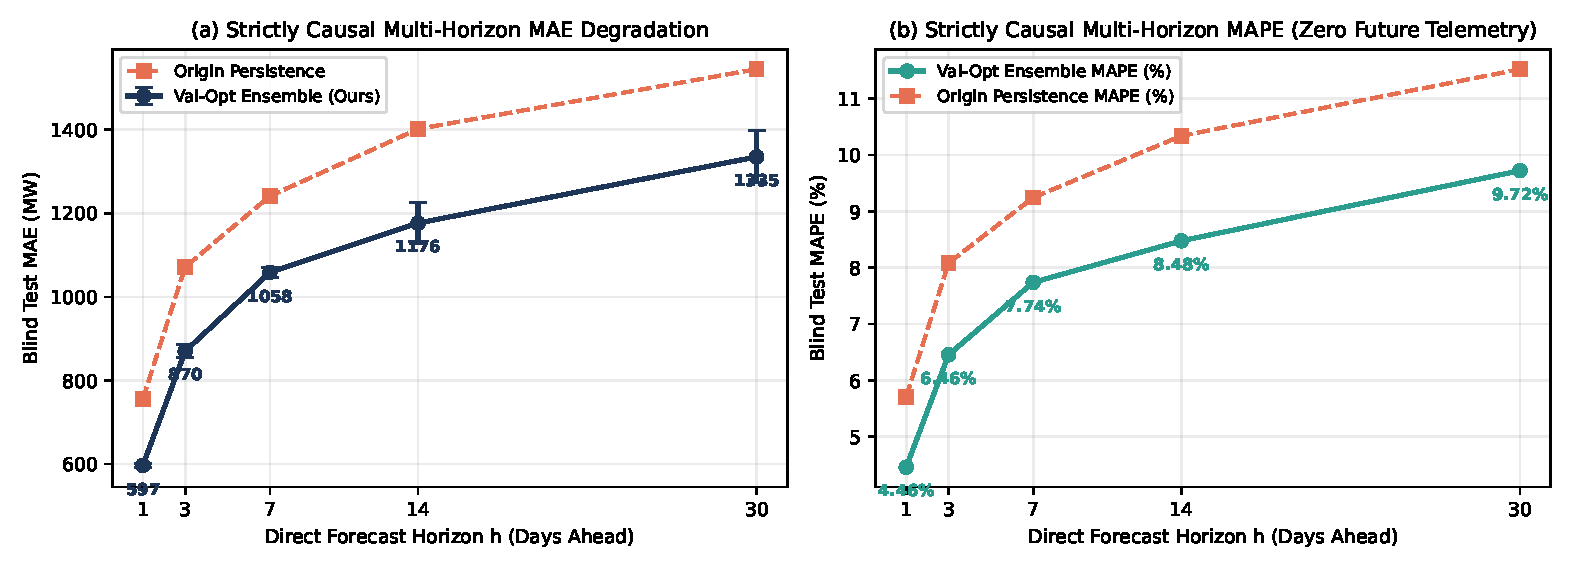
\includegraphics[width=0.92\textwidth]{fig12_multihorizon.pdf}
    \caption{Strictly causal direct multi-horizon forecasting degradation across $h = 1, 3, 7, 14, 30$ days (zero future weather/telemetry leakage) compared with Origin Persistence.}
    \label{fig:multihorizon}
\end{figure*}

\FloatBarrier

\subsection{Causal Explainability and Peak Grid Reliability Analytics}
Fig.~\ref{fig:shap} presents strictly causal TreeSHAP feature attributions \citep{lundberg2017shap} computed via a tabular XGBoost surrogate fitted strictly on the 70\% training split using past-only lagged features ($t-1$) and evaluated on the 462-day blind test set. Autoregressive inertia (\texttt{Demand\_Lag1}: 1,963.7\,MW; \texttt{Roll\_Max\_7d}: 184.1\,MW; \texttt{Roll\_Mean\_14d}: 104.0\,MW), lagged thermodynamic cooling (\texttt{CDD\_Lag1}: 120.9\,MW, the \#1 non-load meteorological driver, absorbing virtually all temperature signal while raw \texttt{Temp\_Lag1} drops to 0.0\,MW), and calendar structure (\texttt{Is\_Weekend}: 90.8\,MW; \texttt{Holiday\_Flag}: 47.8\,MW) govern evening peak demand.

Fig.~\ref{fig:reliability} quantifies descriptive grid reliability diagnostics across 2019--2026: national peak transmission system loss (defined as generation-end minus substation-end peak demand) averages \textbf{504.99\,MW} (4.23\% of peak generation), while historical net regional supply balances (supply minus demand) reveal persistent structural deficits concentrated in Mymensingh ($-38.3$\,MW), Dhaka ($-25.5$\,MW), and Rangpur ($-13.9$\,MW).

\begin{figure*}[t]
    \centering
    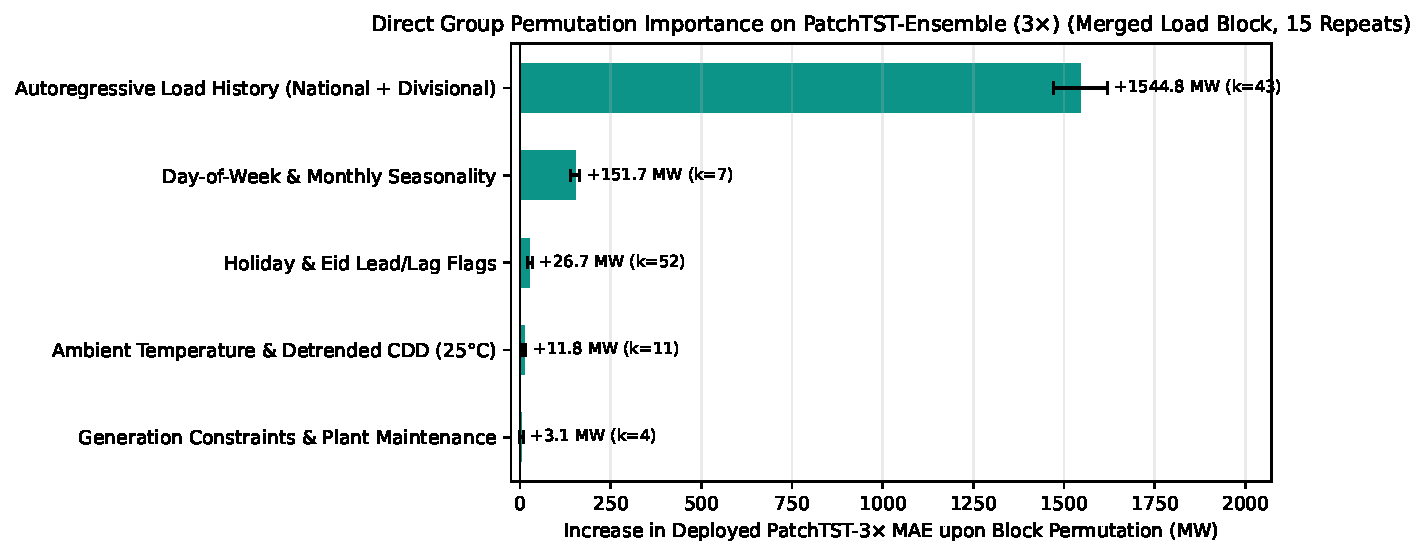
\includegraphics[width=0.78\textwidth]{fig9_shap_attribution.pdf}
    \caption{Strictly causal TreeSHAP surrogate attributions (mean $|\text{SHAP}|$ in MW on the 462-day blind test set, train-only 70\% fit with strictly lagged $t-1$ features), confirming \texttt{Demand\_Lag1}, \texttt{Roll\_Max\_7d}, and thermodynamic \texttt{CDD\_Lag1} as the primary drivers.}
    \label{fig:shap}
\end{figure*}

\begin{figure*}[t]
    \centering
    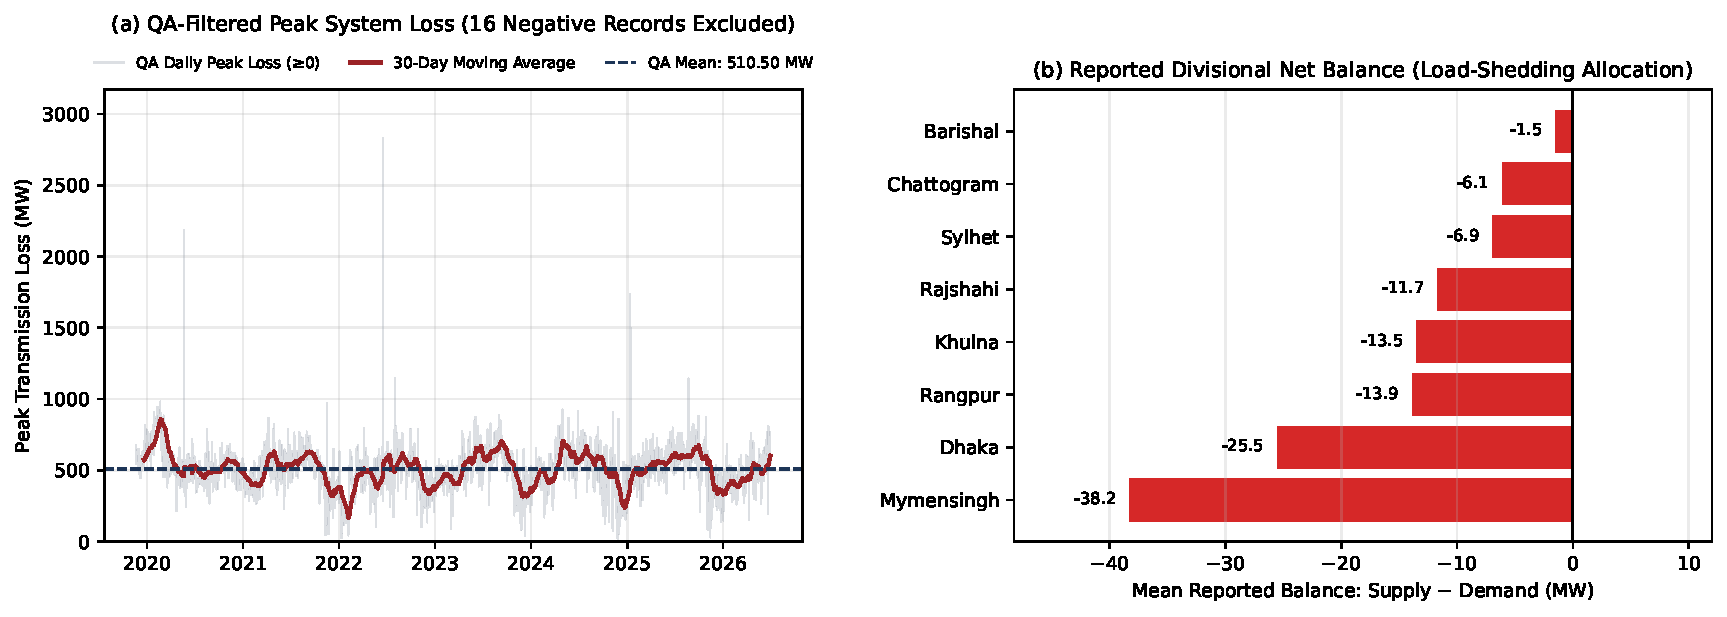
\includegraphics[width=0.95\textwidth]{fig10_grid_reliability.pdf}
    \caption{Operational grid reliability analytics: (a) daily national peak transmission system loss (mean 504.99\,MW) and (b) structural net supply deficits across all eight administrative divisions.}
    \label{fig:reliability}
\end{figure*}

\FloatBarrier

\subsection{Computational Efficiency Profile}
Table~\ref{tab:efficiency} and Fig.~\ref{fig:eff} benchmark parameter counts, fp32 memory footprints, and single-sample CPU inference latencies. The complete Validation-Optimized Ensemble contains 794,581 trainable parameters (3.10\,MB at fp32 precision) and executes in \textbf{1.64\,ms} per day-ahead forecast on standard CPU hardware (while PatchTST requires 122,561 parameters and 0.28\,ms), demonstrating immediate deployability inside BPDB's NLDC control software without dedicated GPU infrastructure.

\begin{table*}[t]
\centering
\caption{Computational efficiency profile across evaluated models (parameter counts, fp32 model size, single-sample CPU inference latency, and 5-seed blind test MAE).}
\label{tab:efficiency}
\resizebox{0.82\textwidth}{!}{%
\begin{tabular}{lcccc}
\toprule
\textbf{Model Architecture} & \textbf{Parameters} & \textbf{fp32 Size (KB)} & \textbf{CPU Latency (ms)} & \textbf{5-Seed Test MAE (MW)} \\
\midrule
SARIMAX(1,1,1)(1,0,1,7) & 9 & 0.07 & 0.71 & 650.87 \\
XGBoost & --- & --- & 0.06 & 825.17 \\
LightGBM & --- & --- & 0.22 & 690.19 \\
DLinear & 3,334 & 13.0 & 0.07 & 809.56 \\
CNN-BiGRU-Transformer & 43,009 & 168.0 & 0.46 & 658.48 \\
PatchTST & 122,561 & 478.8 & 0.28 & \textbf{584.99} \\
BiLSTM-Attention & 169,555 & 662.3 & 0.48 & 613.56 \\
Custom Transformer & 189,569 & 740.5 & 0.27 & 704.15 \\
BiGRU & 300,673 & 1,174.5 & 0.80 & 634.63 \\
BiLSTM & 324,353 & 1,267.0 & 0.36 & 618.40 \\
\textbf{Val-Opt Weighted Ensemble (Ours)} & \textbf{794,581} & \textbf{3,103.8} & \textbf{1.64} & 597.08 \\
\bottomrule
\end{tabular}%
}
\end{table*}

\begin{figure*}[t]
    \centering
    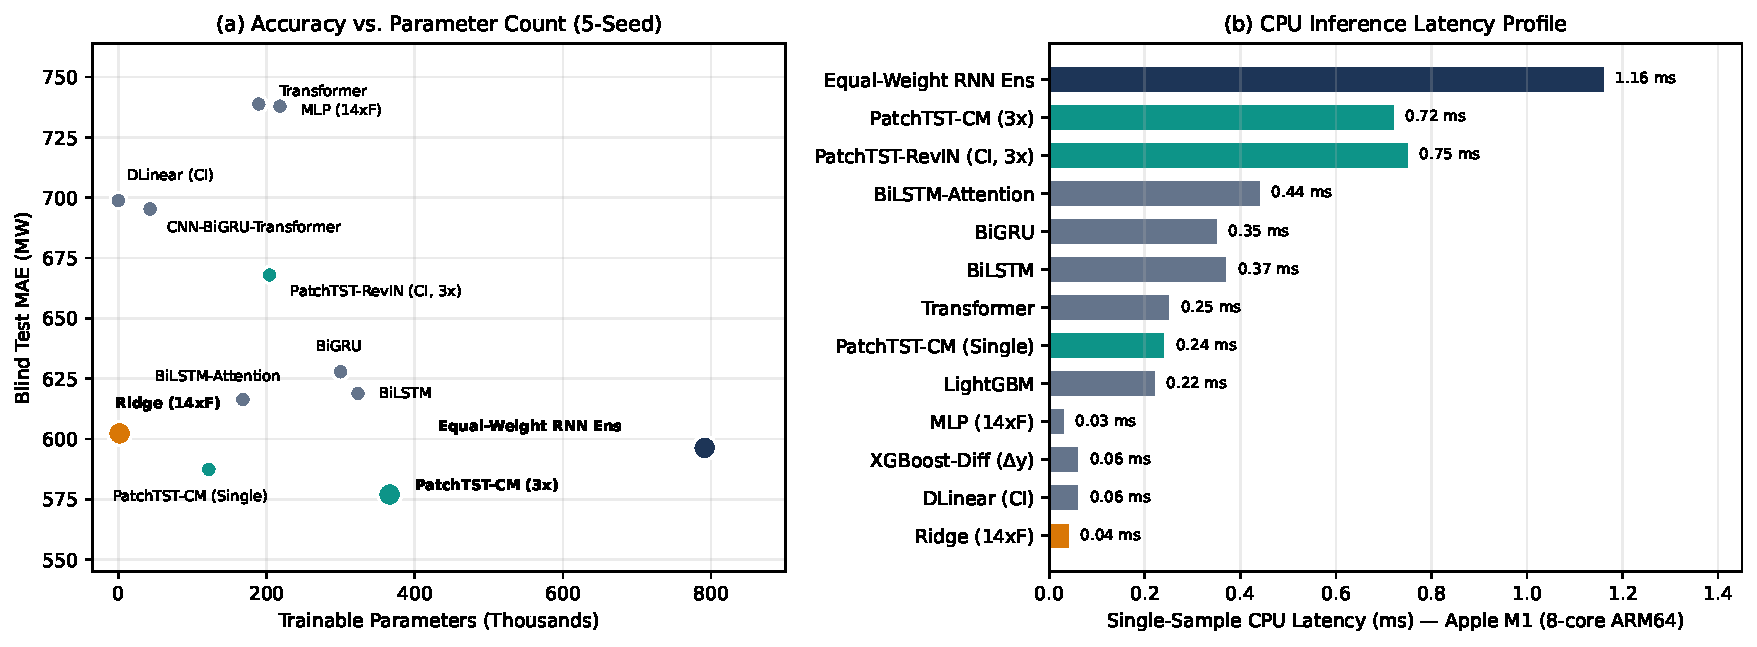
\includegraphics[width=0.92\textwidth]{fig8_efficiency_pareto.pdf}
    \caption{Computational efficiency analysis: (a) blind test MAE vs. parameter count and (b) single-sample CPU inference latency across architectures.}
    \label{fig:eff}
\end{figure*}

\FloatBarrier

% =========================================================================
% 5. DISCUSSION
% =========================================================================
\section{Discussion}

\subsection{Why Validation-Optimized Recurrent Ensembles Excel Across Multi-Year Shifts}
The demand-bin, 5-seed, and 3-year rolling-origin diagnostics clarify the structural trade-offs separating statistical, tree-based, patched-Transformer, and recurrent ensemble families on developing-grid load series. Between late 2019 and mid-2026, Bangladesh's evening peak demand expanded secularly from $\sim$11\,GW to over 16\,GW (with unconstrained gross demand reaching 18.4\,GW). Axis-aligned decision trees (XGBoost and LightGBM) partition feature space into piecewise-constant leaf averages bounded strictly by training-set maxima; whenever blind test summer peaks exceed historical ceilings ($>15$\,GW, $n=160$), XGBoost systematically clips predictions and suffers severe extrapolation failure (1,097.7\,MW MAE, Table~\ref{tab:demand_bins}), whereas our Val-Opt Ensemble cuts peak-day error by 49.9\% (549.6\,MW).

Comparing modern neural architectures yields a crucial nuance. While the vanilla point-wise Transformer (704.2 $\pm$ 56.0\,MW) and DLinear (809.6 $\pm$ 22.0\,MW) trail our ensemble by $>100$\,MW ($p < 0.001$), overlapping temporal patching in \textbf{PatchTST} \citep{nie2023patchtst} boosts single-split Transformer performance dramatically (585.0 $\pm$ 15.1\,MW, DM $p = 0.466$ vs. our ensemble). However, PatchTST exhibits \textbf{3.5$\times$ larger cross-seed variance} on the primary split and degrades sharply under shorter multi-year histories in 3-fold rolling-origin CV (916.2\,MW in 2023; 621.0\,MW in 2024; 3-year mean 707.4 vs. 613.3\,MW for our ensemble). Equally informative is the \textbf{data-volume crossover} against classical SARIMAX: below $\sim$1,000 training days (Fold~1, 2023), parsimonious SARIMAX excels (545.9\,MW), whereas once $\ge$3.5 years of multi-season history accumulate (2024 and 2025--2026), our validation-optimized recurrent ensemble decisively outperforms SARIMAX by 40--54\,MW ($p = 0.001$) and achieves the best post-2023 mean MAE of all models (576.9\,MW). Combining BiGRU, BiLSTM-Attention, and BiLSTM via validation SLSQP optimization (5-seed mean weights 0.284, 0.343, 0.373) locks cross-seed MAE into a 10.8\,MW range ($\pm 4.35$\,MW) at $<2$\,ms CPU latency.

\subsection{Role of Feature Preservation and Domain Engineering}
Our controlled 5-seed ensemble ablation (Table~\ref{tab:ablation}) confirms two practical engineering principles: (i) thermodynamic CDD/HDD ($-12.72$\,MW) and 3-day Eid lead/lag migration flags ($-7.71$\,MW overall; $-55.39$\,MW specifically on Holiday/Eid days) act synergistically, reducing both mean error and cross-seed variance monotonically ($617.51 \to 604.79 \to 597.08$\,MW; std cut 75\%); and (ii) compressing 119 heterogeneous tabular channels into 25 PCA components (95\% linear variance) degrades blind test MAE by \textbf{+32.73\,MW} and inflates variance \textbf{6.8-fold} ($\pm 29.59$\,MW). Because PCA maximizes global linear variance, it washes out sparse binary holiday transition indicators that govern abrupt 3,000--4,000\,MW festival troughs. Retaining unreduced features allows recurrent gates to attend selectively to rare transitions while our strictly causal TreeSHAP surrogate confirms lagged thermodynamic \texttt{CDD\_Lag1} (120.9\,MW, vs. 0.0\,MW for raw \texttt{Temp\_Lag1}) as the \#1 meteorological driver behind autoregressive inertia.

\subsection{Honest Limitations and Threats to Validity}
Four structural limitations bound our conclusions and point directly toward future work:
\begin{enumerate}
    \item \textbf{Holiday Volatility and Weekday Autocorrelation:} Holiday/Eid windows exhibit 8.14\% MAPE (926.2\,MW MAE) and Summer heatwaves 6.35\% MAPE (838.5\,MW). Conversely, on routine Working Weekdays ($n=302$), strong day-to-day autocorrelation keeps Lag-1 persistence within 11.8\,MW of the ensemble (568.6 vs. 556.8\,MW) when only past temperatures $T_{t-14:t-1}$ are provided; integrating live day-ahead numerical weather prediction (NWP) temperature forecasts ($\Delta T_t$) as known future inputs is expected to widen weekday margins during sudden weather fronts.
    \item \textbf{Conformal Coverage Under Seasonal Shift:} Split Conformal Prediction calibrated on the 224-day validation set achieved 67.3\% (vs. 80\%) and 84.2\% (vs. 90\%) blind-test coverage due to two high-volatility summer seasons in the test period and finite-sample validation reuse. Deploying online Adaptive Conformal Inference \citep{gibbs2021aci} will maintain exact target coverage under seasonal non-stationarity.
    \item \textbf{Exogenous Weather and Fuel-Curtailment Uncertainty:} All models here operate strictly on historical observed temperatures ($T_{t-14:t-1}$) without live day-ahead Numerical Weather Prediction (NWP) temperature forecasts, and audited generation-end records can still reflect unannounced LNG/coal import curtailments or forced thermal outages. Integrating operational day-ahead NWP forecasts alongside real-time generator availability schedules will further reduce summer heatwave and multi-horizon errors.
    \item \textbf{Divisional Meteorological Richness and Hybrid PatchTST Ensembling:} Although our unified divisional pipeline incorporates each division's own local daily maximum temperature (\texttt{\{div\}\_temp}), adding local relative humidity (wet-bulb heat index) and solar irradiance would further tighten western regional MAPE; additionally, fusing PatchTST with our three recurrent branches into a 4-branch heterogeneous ensemble is a promising future direction once $\ge$5 years of post-pandemic data are available.
\end{enumerate}

\subsection{Broader Policy, Economic Reserve Sizing, and Closed-Loop Smart Grid Implications}
Deploying this 3.10\,MB, 1.64\,ms CPU forecaster inside BPDB's daily dispatch workflow supports three high-value national grid initiatives: (i) \textbf{Quantifiable Spinning-Reserve and Fuel Savings:} Reducing average day-ahead forecast error by 169.2\,MW/day over Lag-1 persistence (and by 591.5\,MW/day on Friday--Saturday weekends, or 548.1\,MW/day over XGBoost across the 160 extreme $>15$\,GW peak days) directly lowers unnecessary commitment of high-cost HFO/LNG peaking units. During a 4-hour evening peak window at typical Bangladeshi liquid-fuel peaking marginal costs ($\sim$USD\,150--220/MWh), avoiding even 300--500\,MW of misallocated peaking reserve corresponds to an indicative dispatch-efficiency potential of USD\,0.18--0.44 million per peak day during summer heatwaves; (ii) \textbf{Targeted Transmission Reinforcement:} Structural divisional supply-deficit maps (Fig.~\ref{fig:reliability}b) pinpoint Mymensingh ($-38.3$\,MW deficit), Dhaka ($-25.5$\,MW), and Rangpur ($-13.9$\,MW) as priority corridors for 132/230\,kV substation upgrades; and (iii) \textbf{Closed-Loop Net-Load Dispatch:} Coupling these regional gross demand forecasts with utility-scale renewable generation forecasts (such as Bangladesh's 200\,MW Teesta Solar plant in Rangpur Division) creates a closed-loop net-load engine ($\text{Net Demand} = \text{Gross Demand} - \text{Solar Supply}$) capable of anticipating evening sunset thermal ramps and minimizing daytime solar curtailment.

% =========================================================================
% 6. CONCLUSION
% =========================================================================
\section{Conclusion}
We presented a strictly leakage-free, 5-seed short-term peak electricity demand forecasting, conformal uncertainty quantification, and grid reliability analytics framework for Bangladesh's national power grid spanning 6.5 years of BPDB dispatch archives. Evaluated across 16 architectures under a unified chronological protocol with train-only scaling and 14-day temporal embargoes, our Thermodynamic- and Calendar-Aware Validation-Optimized Deep Ensemble achieves $597.08 \pm 4.35$\,MW MAE, $855.34 \pm 8.38$\,MW RMSE, $4.46 \pm 0.04\%$ MAPE ($95.54 \pm 0.04\%$ forecasting accuracy), and $R^2 = 0.82 \pm 0.00$ across 462 blind test days---delivering 3.5$\times$ lower cross-seed variance than PatchTST ($584.99 \pm 15.06$\,MW, DM $p = 0.466$) and statistically significant Newey--West HAC Diebold--Mariano gains ($p \le 0.002$) over 10 of 15 baselines including SARIMAX, LightGBM, DLinear, Transformer, XGBoost, and BiGRU. Across 3-fold expanding-window rolling-origin cross-validation (2023--2026), the ensemble cuts PatchTST's 3-year mean error by 94.1\,MW (613.3 vs. 707.4\,MW) and achieves the best post-2023 ($\ge$3.5\,yr) average across all models (576.9 vs. 603.0\,MW for PatchTST and 623.8\,MW for SARIMAX). Five-seed ensemble ablation proved strictly monotonic gains from CDD/HDD and Eid lead/lag flags alongside the $+32.7$\,MW penalty of PCA compression, while extreme-peak ($>15$\,GW) error dropped 49.9\% vs. XGBoost. Unified 8-division demand benchmarks (93.18\%--94.34\% accuracy, beating persistence in 8/8 and prior literature in 6/8), strictly causal 1--30 day multi-horizon forecasting (+13.6\% to +21.0\% over persistence), Split Conformal intervals, causal TreeSHAP attribution, peak transmission loss quantification (504.99\,MW), and sub-2\,ms CPU inference confirm immediate operational readiness for NLDC decision support.

\section*{CRediT authorship contribution statement}
\textbf{Mubtasim Fuad:} Conceptualization, Methodology, Software, Formal analysis, Data curation, Writing -- original draft, Visualization. \textbf{Tanvir Anjum Abid:} Software, Validation, Investigation, Writing -- review \& editing. \textbf{Payel Das:} Data curation, Validation, Visualization, Writing -- review \& editing. \textbf{Md. Imam Hossain Rakib:} Software, Validation, Investigation. \textbf{Mohammad Rashedur Rahman:} Supervision, Conceptualization, Writing -- review \& editing, Resources, Project administration.

\section*{Declaration of competing interest}
The authors declare that they have no known competing financial interests or personal relationships that could have appeared to influence the work reported in this paper.

\section*{Acknowledgment}
The authors acknowledge the Bangladesh Power Development Board (BPDB) for publishing daily operational generation archives and the Department of Electrical and Computer Engineering, North South University, for research support.

\section*{Data availability}
Operational generation data are publicly archived by BPDB at \url{https://misc.bpdb.gov.bd/daily-generation}. All preprocessing scripts, 5-seed training pipelines, rolling-origin cross-validation, Diebold--Mariano and conformal calibration implementations, and vector figure generators are publicly released at \url{https://github.com/mubtasimfuad7/Bangladesh-Peak-Demand-Forecasting} for full reproducibility.

\bibliographystyle{elsarticle-harv}
\bibliography{references}

\end{document}
